% Font options: 10pm, 11pt, 12pt
% Align headings left instead of center: nocenter
\documentclass[xcolor=x11names,compress]{beamer}\usepackage[]{graphicx}\usepackage[]{color}
% maxwidth is the original width if it is less than linewidth
% otherwise use linewidth (to make sure the graphics do not exceed the margin)
\makeatletter
\def\maxwidth{ %
  \ifdim\Gin@nat@width>\linewidth
    \linewidth
  \else
    \Gin@nat@width
  \fi
}
\makeatother

\definecolor{fgcolor}{rgb}{0.345, 0.345, 0.345}
\newcommand{\hlnum}[1]{\textcolor[rgb]{0.686,0.059,0.569}{#1}}%
\newcommand{\hlstr}[1]{\textcolor[rgb]{0.192,0.494,0.8}{#1}}%
\newcommand{\hlcom}[1]{\textcolor[rgb]{0.678,0.584,0.686}{\textit{#1}}}%
\newcommand{\hlopt}[1]{\textcolor[rgb]{0,0,0}{#1}}%
\newcommand{\hlstd}[1]{\textcolor[rgb]{0.345,0.345,0.345}{#1}}%
\newcommand{\hlkwa}[1]{\textcolor[rgb]{0.161,0.373,0.58}{\textbf{#1}}}%
\newcommand{\hlkwb}[1]{\textcolor[rgb]{0.69,0.353,0.396}{#1}}%
\newcommand{\hlkwc}[1]{\textcolor[rgb]{0.333,0.667,0.333}{#1}}%
\newcommand{\hlkwd}[1]{\textcolor[rgb]{0.737,0.353,0.396}{\textbf{#1}}}%
\let\hlipl\hlkwb

\usepackage{framed}
\makeatletter
\newenvironment{kframe}{%
 \def\at@end@of@kframe{}%
 \ifinner\ifhmode%
  \def\at@end@of@kframe{\end{minipage}}%
  \begin{minipage}{\columnwidth}%
 \fi\fi%
 \def\FrameCommand##1{\hskip\@totalleftmargin \hskip-\fboxsep
 \colorbox{shadecolor}{##1}\hskip-\fboxsep
     % There is no \\@totalrightmargin, so:
     \hskip-\linewidth \hskip-\@totalleftmargin \hskip\columnwidth}%
 \MakeFramed {\advance\hsize-\width
   \@totalleftmargin\z@ \linewidth\hsize
   \@setminipage}}%
 {\par\unskip\endMakeFramed%
 \at@end@of@kframe}
\makeatother

\definecolor{shadecolor}{rgb}{.97, .97, .97}
\definecolor{messagecolor}{rgb}{0, 0, 0}
\definecolor{warningcolor}{rgb}{1, 0, 1}
\definecolor{errorcolor}{rgb}{1, 0, 0}
\newenvironment{knitrout}{}{} % an empty environment to be redefined in TeX

\usepackage{alltt}
%\documentclass[xcolor=x11names,compress,handout]{beamer}
\usepackage[]{graphicx}
\usepackage[]{color}
\usepackage{booktabs}
\usepackage{hyperref}
\usepackage{tikz}
\usepackage{multirow}
\usepackage{multicol}
\usepackage{dcolumn}
\usepackage{bigstrut}
\usepackage{amsmath} 
\usepackage{xcolor,colortbl}
\usepackage{amssymb}
%\newcommand{\done}{\cellcolor{teal}#1}

%% Beamer Layout %%%%%%%%%%%%%%%%%%%%%%%%%%%%%%%%%%
\useoutertheme[subsection=false,shadow]{miniframes}
\useinnertheme{default}
\usefonttheme{serif}
\usepackage{Arev}
\usepackage{pdfpages}

\setbeamerfont{title like}{shape=\scshape}
\setbeamerfont{frametitle}{shape=\scshape, size=\normalsize}

\definecolor{dkblue}{RGB}{0,0,102}

\setbeamercolor*{lower separation line head}{bg=dkblue} 
\setbeamercolor*{normal text}{fg=black,bg=white} 
\setbeamercolor*{alerted text}{fg=red} 
\setbeamercolor*{example text}{fg=black} 
\setbeamercolor*{structure}{fg=black} 
 
\setbeamercolor*{palette tertiary}{fg=black,bg=black!10} 
\setbeamercolor*{palette quaternary}{fg=black,bg=black!10} 

\renewcommand{\(}{\begin{columns}}
\renewcommand{\)}{\end{columns}}
\newcommand{\<}[1]{\begin{column}{#1}}
\renewcommand{\>}{\end{column}}

\setbeamertemplate{navigation symbols}{} 
\setbeamertemplate{footline}[frame number]
\setbeamertemplate{caption}{\raggedright\insertcaption\par}

\setbeamersize{text margin left=5pt,text margin right=5pt}

\AtBeginSection{\frame{\sectionpage}}
\usepackage{xcolor}
\hypersetup{
    colorlinks,
    linkcolor={red!50!black},
    citecolor={blue!50!black},
    urlcolor={blue!80!black}
}

%%%%%%%%%%%%%%%%%%%%%%%%%%%%%%%%%%%%%%%%%%%%%%%%%%







\title{FLS 6441 - Methods III: Explanation and Causation}
\subtitle{Week 1 - Review of Regression}
\author{Jonathan Phillips}
\date{March 2020}
\IfFileExists{upquote.sty}{\usepackage{upquote}}{}
\begin{document}

\frame{\titlepage}

\begin{frame}
\frametitle{Course Objectives}
\begin{enumerate}
\item Change how you think about quantitative methods, \textit{explaining} politics, and not just describing it
\pause
\item Understand the 'toolkit' of causal methods used in top journals
\pause
\item Apply those methods to your own research questions
\pause
\end{enumerate}
\begin{center}
\href{https://jonnyphillips.github.io/Methods_III}{Course Website}
\end{center}
\end{frame}

\begin{frame}
\frametitle{Course Topics}
\begin{enumerate}
\item Review of Regression (5th March)
\pause
\item A Framework for Explanation (12th March)
\pause
\item Field Experiments (19th March)
\item Survey and Lab Experiments (26th March)
\item Randomized Natural Experiments (2nd April, Semana Santa)
\pause
\item Instrumental Variables (16th April)
\item Discontinuities (23rd April)
\pause
\item Difference-in-Differences (30th April)
\item Controlling for Confounding (7th May)
\item Matching (14th May)
\item Comparative Cases and Process Tracing (21st May)
\pause
\item Generalizability, Reproducibility and Mechanisms (28th May)
\end{enumerate}
\end{frame}

\begin{frame}
\frametitle{Course Schedule}
\begin{itemize}
\item Wednesday 18h - Submit Replication Task
\pause
\item Thursday 14h-16h - Room 105
\pause
\item Thursday 16.15-18.00 - Lab 122
\end{itemize}
\end{frame}

\begin{frame}
\frametitle{Evaluation}
\begin{itemize}
\item Replication Tasks - 40\%
\pause
\begin{itemize}
\item 8 best grades out of 10 tasks
\end{itemize}
\pause
\item Short Research Paper - 40\%
\pause
\item Participation - 20\%
\end{itemize}
\end{frame}

\begin{frame}
\frametitle{Short Research Paper}
\begin{itemize}
\item Quality $>$ Quantity
\pause
\item Max 15 pages, English or Portuguese
\pause
\item Submit paper and code by email to me by 24th July 2020
\pause
\item Use at least one of the methods studied in class
\pause
\item \textit{Tip:} Pick a simple \textit{causal} question and dataset
\end{itemize}
\end{frame}

\begin{frame}
\frametitle{If you get Lost:}
\begin{enumerate}
\item Don't panic! Everyone needs to see this content 3 or 4 times to 'get' it
\pause
\item Simplify your thoughts - all the methods are doing \textit{less} than you think they are
\pause
\item Re-read the slides and core readings
\pause
\item Search online
\pause
\item Ask your friends - they can explain better than me
\pause
\item Ask me
\end{enumerate}
\end{frame}

\begin{frame}
\frametitle{Today's Objectives}
\begin{enumerate}
\item What Does Regression Actually Do?
\item Guide to 'Smart' Regression
\item What Does Regression NOT Do?
\end{enumerate}
\end{frame}

\section{What Does Regression Actually Do?}

\begin{frame}
\frametitle{Data}
\begin{itemize}
\item We work with variables, which VARY!
\end{itemize}
\begin{multicols}{2}
% latex table generated in R 3.5.2 by xtable 1.8-3 package
% Sat Mar 16 08:25:14 2019
\begin{table}[ht]
\centering
\begin{tabular}{r}
  \hline
Variable \\ 
  \hline
0.30 \\ 
  -0.67 \\ 
  0.39 \\ 
  0.03 \\ 
  -1.26 \\ 
  1.26 \\ 
  -1.44 \\ 
  0.16 \\ 
  0.50 \\ 
  0.01 \\ 
   \hline
\end{tabular}
\end{table}

\columnbreak
\begin{knitrout}
\definecolor{shadecolor}{rgb}{0.969, 0.969, 0.969}\color{fgcolor}
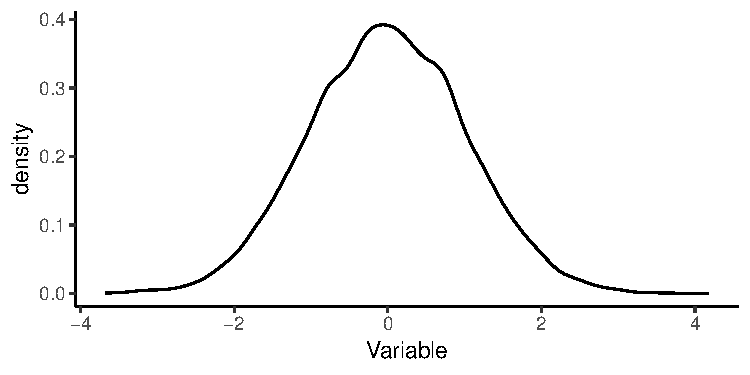
\includegraphics[width=\maxwidth]{figure/var2-1} 

\end{knitrout}
\end{multicols}
\end{frame}

\begin{frame}
\frametitle{Data}
\begin{itemize}
\item We work with variables, which VARY!
\end{itemize}
\begin{multicols}{2}
% latex table generated in R 3.5.2 by xtable 1.8-3 package
% Sat Mar 16 08:28:46 2019
\begin{table}[ht]
\centering
\begin{tabular}{rr}
  \hline
Variable\_1 & Variable\_2 \\ 
  \hline
-0.44 & 0.63 \\ 
  0.06 & 0.68 \\ 
  -0.21 & -0.02 \\ 
  0.44 & -0.25 \\ 
  1.29 & 0.46 \\ 
  -0.38 & -0.81 \\ 
  -1.04 & 0.24 \\ 
  -0.16 & 1.84 \\ 
  1.29 & 0.06 \\ 
  -0.10 & -0.18 \\ 
   \hline
\end{tabular}
\end{table}

\columnbreak
\begin{knitrout}
\definecolor{shadecolor}{rgb}{0.969, 0.969, 0.969}\color{fgcolor}
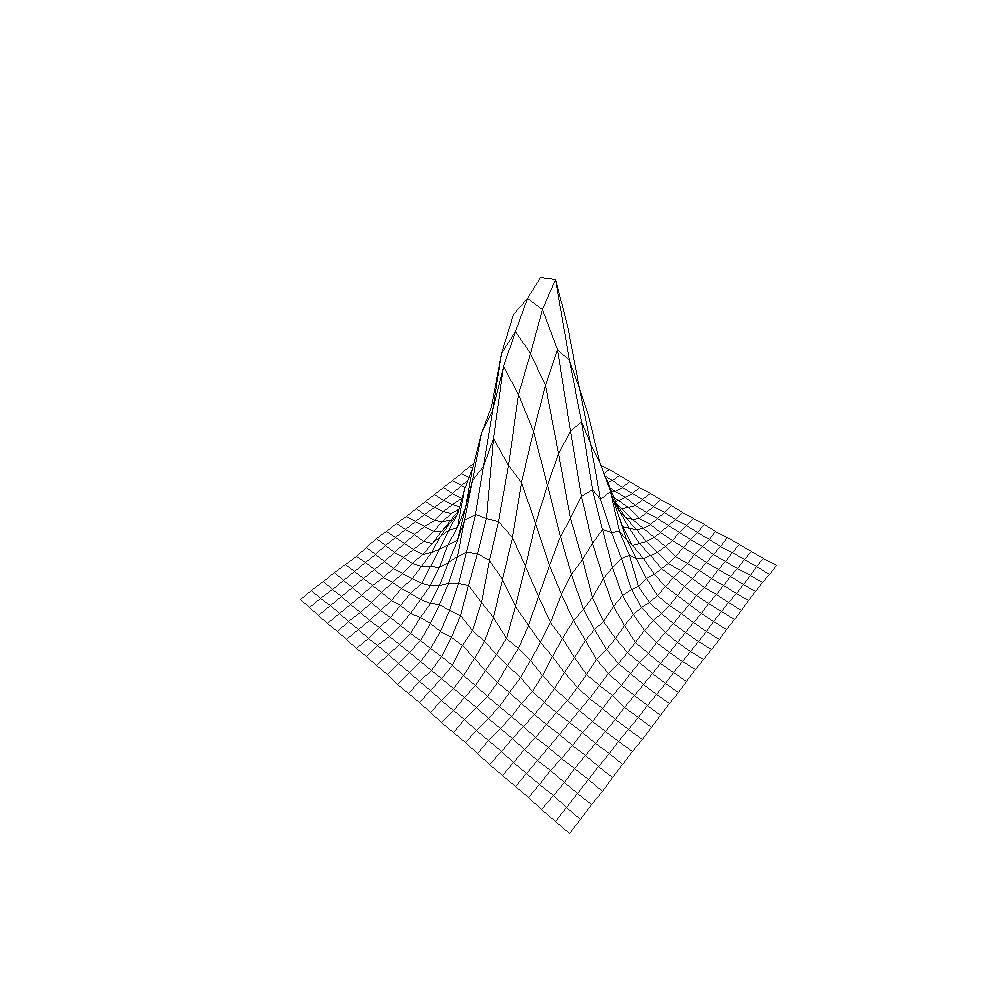
\includegraphics[width=\maxwidth]{figure/var4-1} 

\end{knitrout}
\end{multicols}
\end{frame}

\begin{frame}
\frametitle{Data}
\begin{itemize}
\item We work with variables, which VARY!
\end{itemize}
\begin{multicols}{2}
% latex table generated in R 3.5.2 by xtable 1.8-3 package
% Thu Mar 21 09:13:31 2019
\begin{table}[ht]
\centering
\begin{tabular}{rr}
  \hline
Variable\_1 & Variable\_2 \\ 
  \hline
-0.86 & -0.69 \\ 
  -0.35 & -0.44 \\ 
  1.27 & 0.42 \\ 
  -0.35 & -0.22 \\ 
  -0.43 & -0.56 \\ 
  0.05 & -0.04 \\ 
  0.69 & 0.70 \\ 
  1.27 & 1.07 \\ 
  0.22 & -0.00 \\ 
  -0.28 & -0.13 \\ 
   \hline
\end{tabular}
\end{table}

\columnbreak
\begin{knitrout}
\definecolor{shadecolor}{rgb}{0.969, 0.969, 0.969}\color{fgcolor}
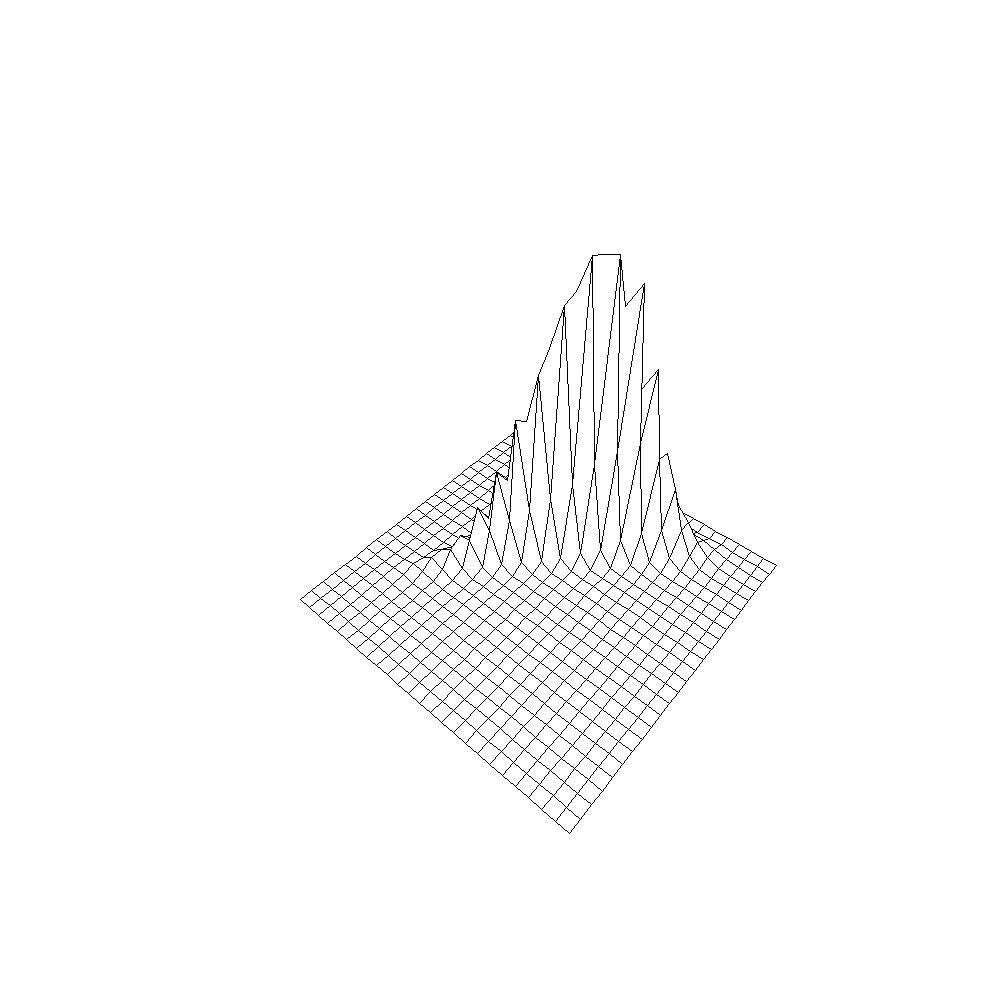
\includegraphics[width=\maxwidth]{figure/var6-1} 

\end{knitrout}
\end{multicols}
\end{frame}




\begin{frame}
\frametitle{What Does Regression Actually Do?}
\begin{enumerate}
\item Regression as Least Squares
\item Regression as Conditional Expectation
\item Regression as (Partial) Correlation
\end{enumerate}
\end{frame}


\begin{frame}
\frametitle{1. Regression as Least Squares}
\begin{itemize}
\item Regression identifies the line through the data that minimizes the sum of squared vertical distances 
\pause
\item $y_i = \alpha + \beta D_i + \epsilon_i$
\pause
\end{itemize}
\begin{multicols}{2}
\begin{knitrout}
\definecolor{shadecolor}{rgb}{0.969, 0.969, 0.969}\color{fgcolor}
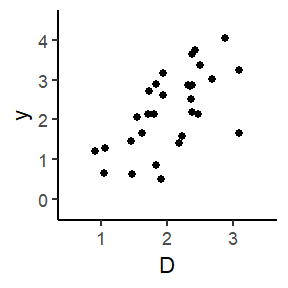
\includegraphics[width=\maxwidth]{figure/graph_ols0-1} 

\end{knitrout}
\columnbreak
 
\end{multicols}
\end{frame}

\begin{frame}
\frametitle{1. Regression as Least Squares}
\begin{itemize}
\item Regression identifies the line through the data that minimizes the sum of squared vertical distances 
\item $y_i = \alpha + \beta D_i + \epsilon_i$
\end{itemize}
\begin{multicols}{2}
\begin{knitrout}
\definecolor{shadecolor}{rgb}{0.969, 0.969, 0.969}\color{fgcolor}
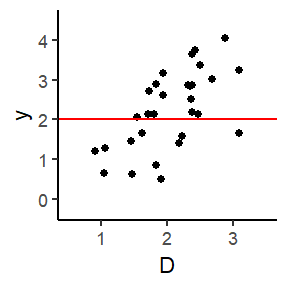
\includegraphics[width=\maxwidth]{figure/graph_ols0b-1} 

\end{knitrout}
\columnbreak
 
\end{multicols}
\end{frame}

\begin{frame}
\frametitle{1. Regression as Least Squares}
\begin{itemize}
\item Regression identifies the line through the data that minimizes the sum of squared vertical distances 
\item $y_i = \alpha + \beta D_i + \epsilon_i$
\end{itemize}
\begin{multicols}{2}
Slope = 0
\begin{knitrout}
\definecolor{shadecolor}{rgb}{0.969, 0.969, 0.969}\color{fgcolor}
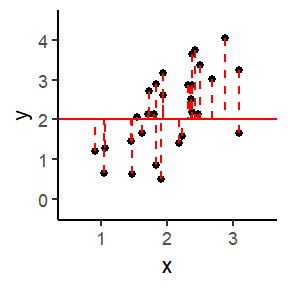
\includegraphics[width=\maxwidth]{figure/graph_ols1-1} 

\end{knitrout}
\columnbreak
\pause
Sum of Residuals$^2$ = 29.6
\begin{knitrout}
\definecolor{shadecolor}{rgb}{0.969, 0.969, 0.969}\color{fgcolor}
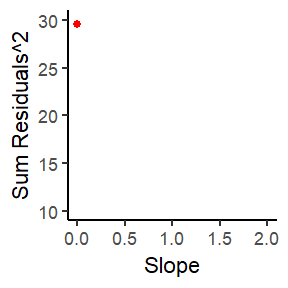
\includegraphics[width=\maxwidth]{figure/graph_ssr1-1} 

\end{knitrout}
\end{multicols}
\end{frame}

\begin{frame}
\frametitle{1. Regression as Least Squares}
\begin{itemize}
\item Regression identifies the line through the data that minimizes the sum of squared vertical distances 
\item $y_i = \alpha + \beta D_i + \epsilon_i$
\end{itemize}
\begin{multicols}{2}
Slope = 0.5
\begin{knitrout}
\definecolor{shadecolor}{rgb}{0.969, 0.969, 0.969}\color{fgcolor}
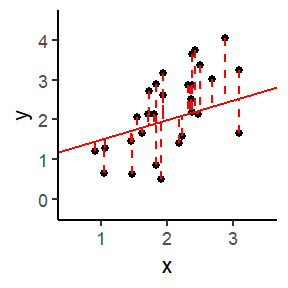
\includegraphics[width=\maxwidth]{figure/graph_ols2-1} 

\end{knitrout}
\columnbreak
Sum of Residuals$^2$ = 21.6
\begin{knitrout}
\definecolor{shadecolor}{rgb}{0.969, 0.969, 0.969}\color{fgcolor}
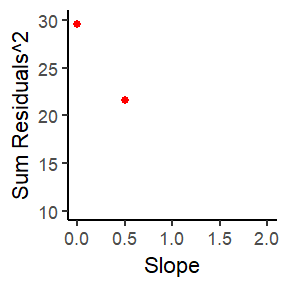
\includegraphics[width=\maxwidth]{figure/graph_ssr2-1} 

\end{knitrout}
\end{multicols}
\end{frame}

\begin{frame}
\frametitle{1. Regression as Least Squares}
\begin{itemize}
\item Regression identifies the line through the data that minimizes the sum of squared vertical distances 
\item $y_i = \alpha + \beta D_i + \epsilon_i$
\end{itemize}
\begin{multicols}{2}
Slope = 1
\begin{knitrout}
\definecolor{shadecolor}{rgb}{0.969, 0.969, 0.969}\color{fgcolor}
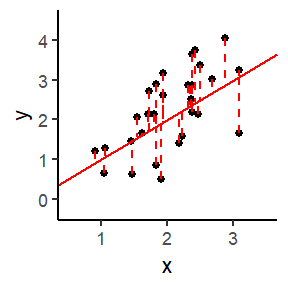
\includegraphics[width=\maxwidth]{figure/graph_ols3-1} 

\end{knitrout}
\columnbreak
Sum of Residuals$^2$ = 18.3
\begin{knitrout}
\definecolor{shadecolor}{rgb}{0.969, 0.969, 0.969}\color{fgcolor}
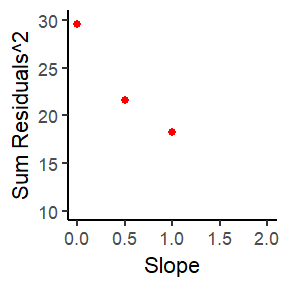
\includegraphics[width=\maxwidth]{figure/graph_ssr3-1} 

\end{knitrout}
\end{multicols}
\end{frame}

\begin{frame}
\frametitle{1. Regression as Least Squares}
\begin{itemize}
\item Regression identifies the line through the data that minimizes the sum of squared vertical distances 
\item $y_i = \alpha + \beta D_i + \epsilon_i$
\end{itemize}
\begin{multicols}{2}
Slope = 1.5
\begin{knitrout}
\definecolor{shadecolor}{rgb}{0.969, 0.969, 0.969}\color{fgcolor}
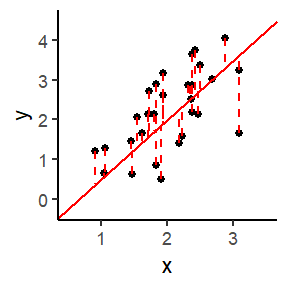
\includegraphics[width=\maxwidth]{figure/graph_ols4-1} 

\end{knitrout}
\columnbreak
Sum of Residuals$^2$ = 19.6
\begin{knitrout}
\definecolor{shadecolor}{rgb}{0.969, 0.969, 0.969}\color{fgcolor}
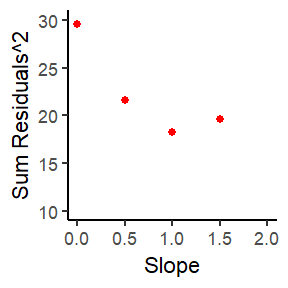
\includegraphics[width=\maxwidth]{figure/graph_ssr4-1} 

\end{knitrout}
\end{multicols}
\end{frame}

\begin{frame}
\frametitle{1. Regression as Least Squares}
\begin{itemize}
\item Regression identifies the line through the data that minimizes the sum of squared vertical distances 
\item $y_i = \alpha + \beta D_i + \epsilon_i$
\end{itemize}
\begin{multicols}{2}
Slope = 2
\begin{knitrout}
\definecolor{shadecolor}{rgb}{0.969, 0.969, 0.969}\color{fgcolor}
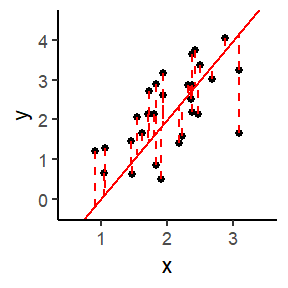
\includegraphics[width=\maxwidth]{figure/graph_ols5-1} 

\end{knitrout}
\columnbreak
Sum of Residuals$^2$ = 25.5
\begin{knitrout}
\definecolor{shadecolor}{rgb}{0.969, 0.969, 0.969}\color{fgcolor}
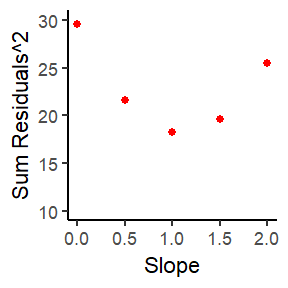
\includegraphics[width=\maxwidth]{figure/graph_ssr5-1} 

\end{knitrout}
\end{multicols}
\end{frame}

\begin{frame}
\frametitle{1. Regression as Least Squares}
\begin{itemize}
\item Regression identifies the line through the data that minimizes the sum of squared vertical distances 
\item $y_i = \alpha + \beta D_i + \epsilon_i$
\end{itemize}
\begin{multicols}{2}
Slope = 1
\begin{knitrout}
\definecolor{shadecolor}{rgb}{0.969, 0.969, 0.969}\color{fgcolor}
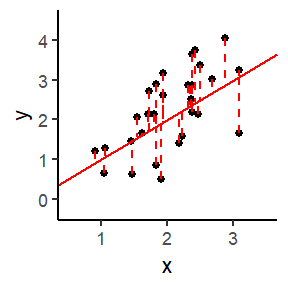
\includegraphics[width=\maxwidth]{figure/graph_ols6-1} 

\end{knitrout}
\columnbreak
Sum of Residuals$^2$ = 18.3
\begin{knitrout}
\definecolor{shadecolor}{rgb}{0.969, 0.969, 0.969}\color{fgcolor}
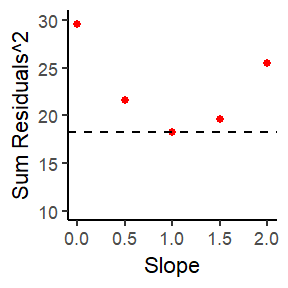
\includegraphics[width=\maxwidth]{figure/graph_ssr6-1} 

\end{knitrout}
\end{multicols}
\end{frame}

%Add noise
\begin{frame}
\frametitle{1. Regression as Least Squares}
\begin{itemize}
\item If we add pure \textit{noise} to $y$, our estimate of $\beta$ is unchanged
\pause
\begin{itemize}
\item The residual error increases
\end{itemize}
\item $y_i = \alpha + \beta D_i + \epsilon_i$
\end{itemize}
\begin{multicols}{2}
Slope = 1
\begin{knitrout}
\definecolor{shadecolor}{rgb}{0.969, 0.969, 0.969}\color{fgcolor}
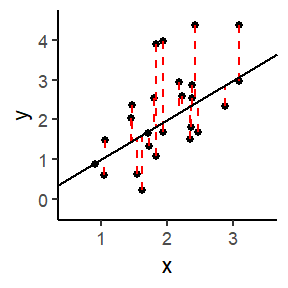
\includegraphics[width=\maxwidth]{figure/graph_ols7-1} 

\end{knitrout}
\columnbreak
\pause
Sum of Residuals$^2$ = 63.9
\begin{knitrout}
\definecolor{shadecolor}{rgb}{0.969, 0.969, 0.969}\color{fgcolor}
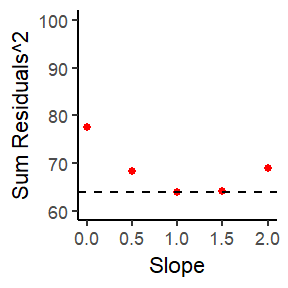
\includegraphics[width=\maxwidth]{figure/graph_ssr7-1} 

\end{knitrout}
\end{multicols}
\end{frame}

\begin{frame}
\frametitle{1. Regression as Least Squares}
\begin{itemize}
\item Dummy control variables \textit{remove variation} associated with specific levels or categories
\begin{itemize}
\item The same as Fixed Effects
\pause
\end{itemize}
\item $y_{ij} = \alpha + \beta_1 D_{ij} + \epsilon_i$
\end{itemize}
\begin{multicols}{2}
\begin{knitrout}
\definecolor{shadecolor}{rgb}{0.969, 0.969, 0.969}\color{fgcolor}
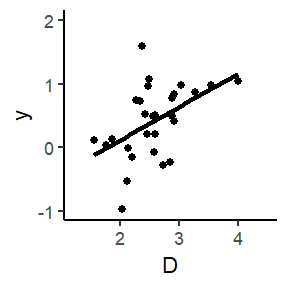
\includegraphics[width=\maxwidth]{figure/graph_ols_FE1-1} 

\end{knitrout}
\columnbreak
Ignoring the dummy control variable, the slope coefficient is 1 
\end{multicols}
\end{frame}

\begin{frame}
\frametitle{1. Regression as Least Squares}
\begin{itemize}
\item Dummy control variables \textit{remove variation} associated with specific levels or categories
\begin{itemize}
\item The same for fixed effects
\end{itemize}
\item $y_{ij} = \alpha + \beta_1 D_{ij} + \epsilon_i$
\end{itemize}
\begin{multicols}{2}
\begin{knitrout}
\definecolor{shadecolor}{rgb}{0.969, 0.969, 0.969}\color{fgcolor}
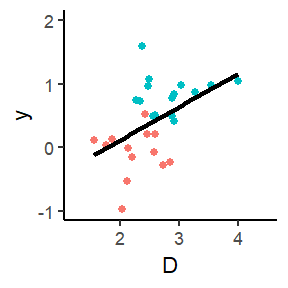
\includegraphics[width=\maxwidth]{figure/graph_ols_FE2-1} 

\end{knitrout}
\columnbreak
But the data points really represent two very different groups, blues and reds
\end{multicols}
\end{frame}

\begin{frame}
\frametitle{1. Regression as Least Squares}
\begin{itemize}
\item Dummy control variables \textit{remove variation} associated with specific levels or categories
\begin{itemize}
\item The same for fixed effects
\end{itemize}
\item $y_{ij} = \alpha + \beta_1 D_{ij} + \beta_2 X_j + \epsilon_i$
\end{itemize}
\begin{multicols}{2}
\begin{knitrout}
\definecolor{shadecolor}{rgb}{0.969, 0.969, 0.969}\color{fgcolor}
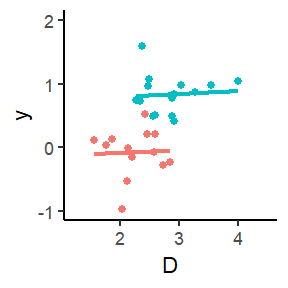
\includegraphics[width=\maxwidth]{figure/graph_ols_FE3-1} 

\end{knitrout}
\columnbreak
What if we ran the regression for each group \textit{separately}?
\end{multicols}
\end{frame}

\begin{frame}
\frametitle{1. Regression as Least Squares}
\begin{itemize}
\item Dummy control variables \textit{remove variation} associated with specific levels or categories
\begin{itemize}
\item The same for fixed effects
\end{itemize}
\item $y_{ij} = \alpha + \beta_1 D_{ij} + \beta_2 X_j + \epsilon_i$
\end{itemize}
\begin{multicols}{2}
\begin{knitrout}
\definecolor{shadecolor}{rgb}{0.969, 0.969, 0.969}\color{fgcolor}
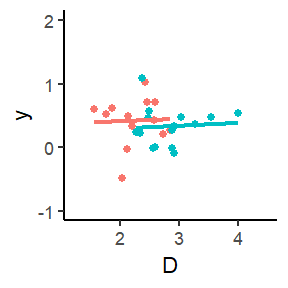
\includegraphics[width=\maxwidth]{figure/graph_ols_FE4-1} 

\end{knitrout}
\columnbreak
Dummy control variables \textit{remove} the average $Y$ differences between blues and reds
\end{multicols}
\end{frame}

\begin{frame}
\frametitle{1. Regression as Least Squares}
\begin{itemize}
\item Dummy control variables \textit{remove variation} associated with specific levels or categories
\begin{itemize}
\item The same for fixed effects
\end{itemize}
\item $y_{ij} = \alpha + \beta_1 D_{ij} + \beta_2 X_j + \epsilon_i$
\end{itemize}
\begin{multicols}{2}
\begin{knitrout}
\definecolor{shadecolor}{rgb}{0.969, 0.969, 0.969}\color{fgcolor}
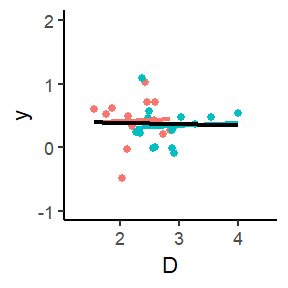
\includegraphics[width=\maxwidth]{figure/graph_ols_FE5-1} 

\end{knitrout}
\columnbreak
The new regression line for the full data now has a slope of zero
\end{multicols}
\end{frame}

\begin{frame}
\frametitle{1. Regression as Least Squares}
\begin{itemize}
\item Dummy control variables \textit{remove variation} associated with specific levels or categories
\begin{itemize}
\item The same for fixed effects
\end{itemize}
\item $y_{ij} = \alpha + \beta_1 D_{ij} + \beta_2 X_j + \epsilon_i$
\end{itemize}
\begin{multicols}{2}
\begin{knitrout}
\definecolor{shadecolor}{rgb}{0.969, 0.969, 0.969}\color{fgcolor}
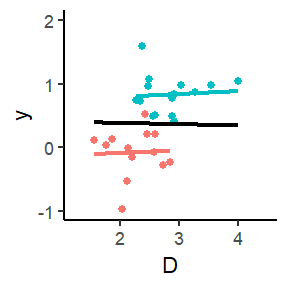
\includegraphics[width=\maxwidth]{figure/graph_ols_FE_last-1} 

\end{knitrout}
\columnbreak
\footnotesize
Equivalently, dummy control variables restrict comparisons to \textbf{within the same group}:
\begin{enumerate}
\item How much does $D$ affect $Y$ within the blue group? 0
\item How much does $D$ affect $Y$ within the red group? 0
\item What's the average of (1) and (2) (weighted by the number of units in each group)? 0
\normalsize
\end{enumerate}
\end{multicols}
\end{frame}

\begin{frame}
\frametitle{1. Regression as Least Squares}
\begin{itemize}
\item Continuous control variables \textit{remove variation} based on how much the control explains $y$
\pause
\item $y_i = \alpha + \beta_1 D_i + \epsilon_i$
\end{itemize}
\begin{multicols}{2}
\begin{knitrout}
\definecolor{shadecolor}{rgb}{0.969, 0.969, 0.969}\color{fgcolor}
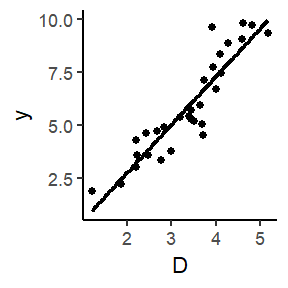
\includegraphics[width=\maxwidth]{figure/graph_ols_control1-1} 

\end{knitrout}
\columnbreak
\pause

The coefficient $\beta_1$ is 2.267 \\
Real effect = 1
\end{multicols}
\end{frame}

\begin{frame}
\frametitle{1. Regression as Least Squares}
\begin{itemize}
\item Continuous control variables \textit{remove variation} based on how much the control explains $y$
\item $y_i = \alpha + \beta_1 D_i + \epsilon_i$
\end{itemize}
\begin{multicols}{2}
\begin{knitrout}
\definecolor{shadecolor}{rgb}{0.969, 0.969, 0.969}\color{fgcolor}
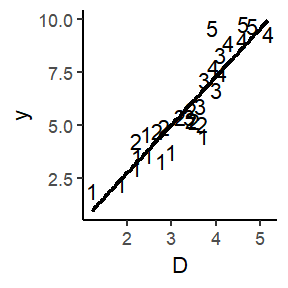
\includegraphics[width=\maxwidth]{figure/graph_ols_control2-1} 

\end{knitrout}
\columnbreak
The coefficient $\beta_1$ is 2.267 \\
Real effect = 1
\end{multicols}
\end{frame}

\begin{frame}
\frametitle{1. Regression as Least Squares}
\begin{itemize}
\item Continuous control variables \textit{remove variation} based on how much the control explains $y$
\item $y_i = \alpha + \beta_1 D_i + \beta_2 X_i + \epsilon_i$
\end{itemize}
\begin{multicols}{2}
\begin{knitrout}
\definecolor{shadecolor}{rgb}{0.969, 0.969, 0.969}\color{fgcolor}
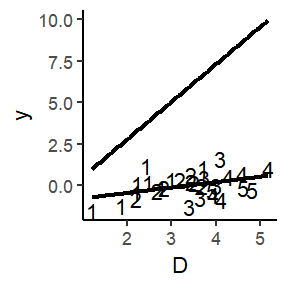
\includegraphics[width=\maxwidth]{figure/graph_ols_control3-1} 

\end{knitrout}
\columnbreak

The coefficient $\beta_1$ is 1.024 \\
Real effect = 1
\end{multicols}
\end{frame}

\begin{frame}
\frametitle{1. Regression as Least Squares}
\begin{itemize}
\item Continuous control variables \textit{remove variation} based on how much the control explains $y$
\item $y_i = \alpha + \beta_1 D_i + \beta_2 X_i + \epsilon_i$
\end{itemize}
\begin{multicols}{2}
\begin{knitrout}
\definecolor{shadecolor}{rgb}{0.969, 0.969, 0.969}\color{fgcolor}
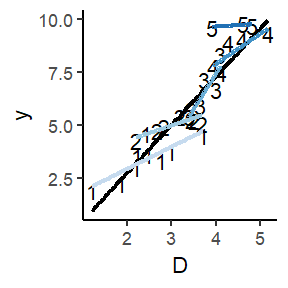
\includegraphics[width=\maxwidth]{figure/graph_ols_control4-1} 

\end{knitrout}
\columnbreak

\begin{itemize}
\item Equivalently, we subset the data to each value of $X$, and find each slope
\pause
\item Then average these slopes, $\beta_1 \sim 1$
\pause
\item Impossible with truly continuous variables
\pause
\item So regression uses linearity to fill in the gaps
\end{itemize}
\end{multicols}
\end{frame}

\begin{frame}
\frametitle{2. Regression as Conditional Expectation}
\begin{itemize}
\item Regression is also a \textbf{Conditional Expectation Function}
\pause
\item \textbf{Conditional on D,} What is our expectation (mean value) of $y$?
\end{itemize}
\small
\begin{center}
\item $y_i = \alpha + \beta_1 D_i + \epsilon_i$ \\
\pause
\item $E(y) = \alpha + \beta_1 D$ \\
\end{center}
\normalsize
\end{frame}

\begin{frame}
\frametitle{2. Regression as Conditional Expectation}
\begin{itemize}
\item \textbf{Conditional on a specific value of D,} what is our expectation (mean value) of $y$?
\end{itemize}
\small
\begin{center}
\item $y_i = \alpha + \beta_1 D_i + \epsilon_i$ \\
\pause
\item $Attitude_i = \alpha + \beta_1 Income_i + N(0,\sigma^2)$ \\
\pause
\item $Attitude_i = 2.235 - 0.000818 * Income_i + N(0,2.38)$ \\
\pause
\item $(Attitude_i | Income_i=3000) = 2.235 - 0.000818 * 3000 + N(0,2.38)$ \\
\pause
\item $(Attitude_i | Income_i=3000) = -0.22 + N(0,2.38)$ \\
\pause
\item $E(Attitude | Income=3000) = -0.22$
\end{center}
\normalsize
\end{frame}

\begin{frame}
\frametitle{2. Regression as Conditional Expectation}
\begin{itemize}
\item \textbf{Conditional on a specific value of D,} what is our expectation (mean value) of $y$?
\end{itemize}
\small
\begin{center}
\item $y_i = \alpha + \beta_1 D_i + \epsilon_i$
\item $Attitude_i = \alpha + \beta_1 Income_i + N(0,\sigma^2)$
\item $Attitude_i = 2.235 - 0.000818 * Income_i + N(0,2.38)$
\end{center}
\normalsize
\pause
\begin{itemize}
\item $E(Attitude | Income)$
\begin{itemize}
\item When income is 3000, the average attitude is -0.22
\pause
\item When income  is 6000, the average attitude is -2.67
\pause
\item When income  is -1000, the average attitude is 3.05
\end{itemize}
\pause
\item $E(Attitude|\text{Income, Age, Gender, Municipality})$
\end{itemize}
\end{frame}

\begin{frame}
\frametitle{2. Regression as Conditional Expectation}
\begin{knitrout}
\definecolor{shadecolor}{rgb}{0.969, 0.969, 0.969}\color{fgcolor}
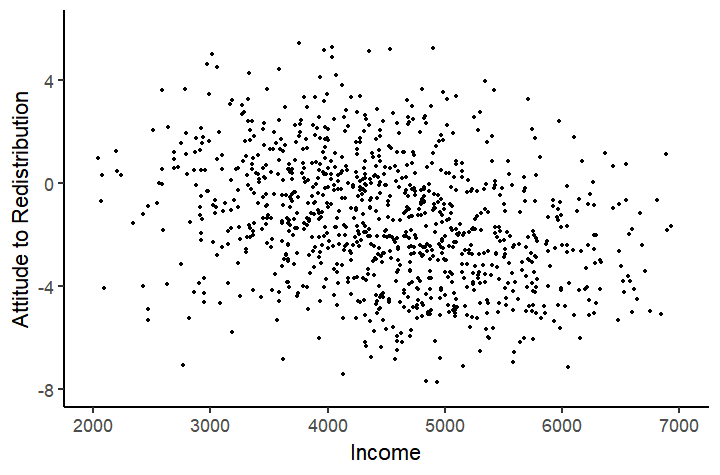
\includegraphics[width=\maxwidth]{figure/cond_exp1a-1} 

\end{knitrout}
\end{frame}

\begin{frame}
\frametitle{2. Regression as Conditional Expectation}
\begin{knitrout}
\definecolor{shadecolor}{rgb}{0.969, 0.969, 0.969}\color{fgcolor}
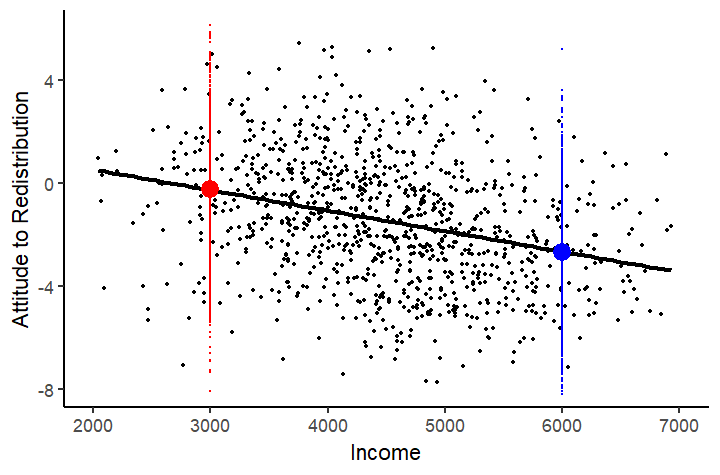
\includegraphics[width=\maxwidth]{figure/cond_exp1b-1} 

\end{knitrout}
\end{frame}

\begin{frame}
\frametitle{2. Regression as Conditional Expectation}
\begin{knitrout}
\definecolor{shadecolor}{rgb}{0.969, 0.969, 0.969}\color{fgcolor}
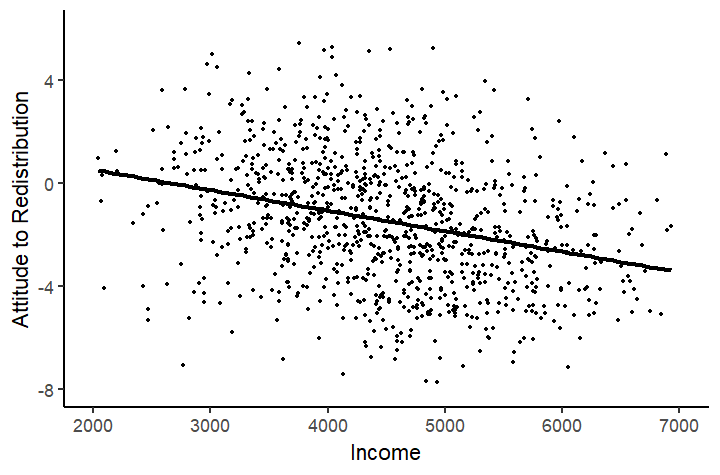
\includegraphics[width=\maxwidth]{figure/cond_exp1c-1} 

\end{knitrout}
\end{frame}


\begin{frame}
\frametitle{2. Regression as Conditional Expectation}
\begin{knitrout}
\definecolor{shadecolor}{rgb}{0.969, 0.969, 0.969}\color{fgcolor}
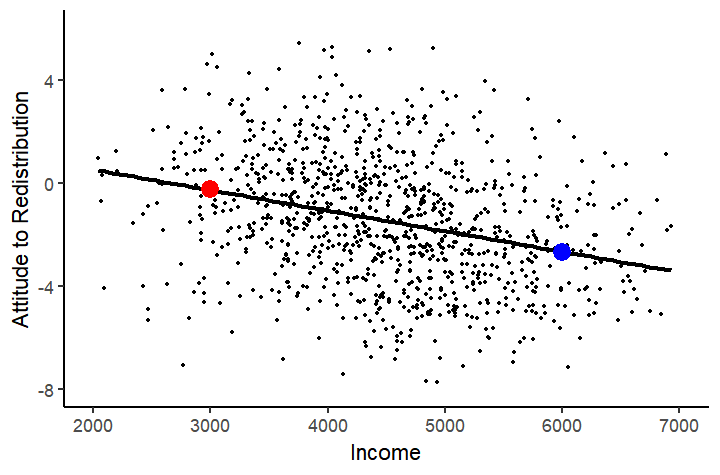
\includegraphics[width=\maxwidth]{figure/cond_exp1-1} 

\end{knitrout}
\end{frame}

\begin{frame}
\frametitle{2. Regression as Conditional Expectation}
\begin{knitrout}
\definecolor{shadecolor}{rgb}{0.969, 0.969, 0.969}\color{fgcolor}
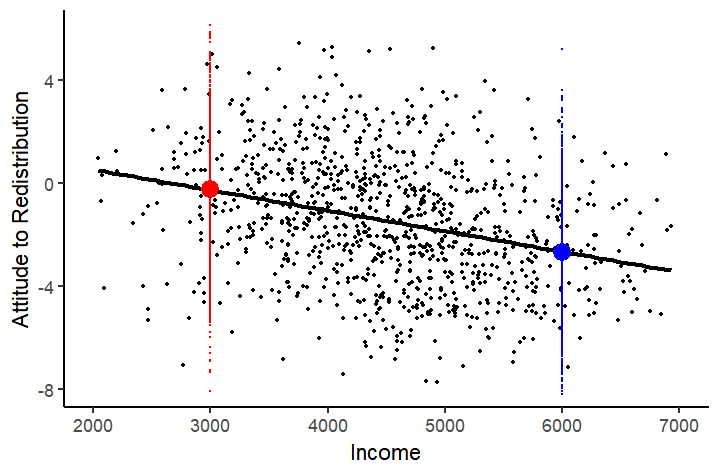
\includegraphics[width=\maxwidth]{figure/cond_exp1b2-1} 

\end{knitrout}
\end{frame}

\begin{frame}
\frametitle{2. Regression as Conditional Expectation}
\begin{itemize}
\item How do we work out the conditional expectation? We estimate the $\beta$s
\pause
\item But we \textbf{NEVER} know the exact value of $\beta$
\pause
\item Regression \textbf{estimates a distribution} for each $\beta$
\pause
\begin{itemize}
\item That's why every $\beta$ comes with a standard error
\pause
\end{itemize}
\end{itemize}
\begin{multicols}{2}

% Table created by stargazer v.5.2.2 by Marek Hlavac, Harvard University. E-mail: hlavac at fas.harvard.edu
% Date and time: Thu, Mar 21, 2019 - 9:36:22 AM
\begin{table}[!htbp] \centering 
  \caption{} 
  \label{} 
\tiny 
\begin{tabular}{@{\extracolsep{1pt}}lc} 
\\[-1.8ex]\hline 
\hline \\[-1.8ex] 
 & \multicolumn{1}{c}{\textit{Dependent variable:}} \\ 
\cline{2-2} 
\\[-1.8ex] & redist \\ 
\hline \\[-1.8ex] 
 income & $-$0.000818$^{***}$ (0.000078) \\ 
  Constant & 2.234719$^{***}$ (0.361477) \\ 
 \hline \\[-1.8ex] 
Observations & 1,000 \\ 
\hline 
\hline \\[-1.8ex] 
\textit{Note:}  & \multicolumn{1}{r}{$^{*}$p$<$0.1; $^{**}$p$<$0.05; $^{***}$p$<$0.01} \\ 
\end{tabular} 
\end{table} 

\columnbreak
\begin{knitrout}
\definecolor{shadecolor}{rgb}{0.969, 0.969, 0.969}\color{fgcolor}
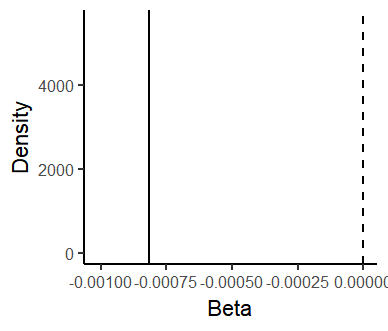
\includegraphics[width=\maxwidth]{figure/beta_dist_a-1} 

\end{knitrout}
\end{multicols}
\end{frame}

\begin{frame}
\frametitle{2. Regression as Conditional Expectation}
\begin{itemize}
\item How do we work out the conditional expectation? We estimate the $\beta$s
\item But we \textbf{NEVER} know the exact value of $\beta$
\item Regression \textbf{estimates a distribution} for each $\beta$
\begin{itemize}
\item That's why every $\beta$ comes with a standard error
\end{itemize}
\end{itemize}
\begin{multicols}{2}

% Table created by stargazer v.5.2.2 by Marek Hlavac, Harvard University. E-mail: hlavac at fas.harvard.edu
% Date and time: Thu, Mar 07, 2019 - 12:50:31 PM
\begin{table}[!htbp] \centering 
  \caption{} 
  \label{} 
\tiny 
\begin{tabular}{@{\extracolsep{1pt}}lc} 
\\[-1.8ex]\hline 
\hline \\[-1.8ex] 
 & \multicolumn{1}{c}{\textit{Dependent variable:}} \\ 
\cline{2-2} 
\\[-1.8ex] & redist \\ 
\hline \\[-1.8ex] 
 income & $-$0.000818$^{***}$ (0.000078) \\ 
  Constant & 2.234719$^{***}$ (0.361477) \\ 
 \hline \\[-1.8ex] 
Observations & 1,000 \\ 
\hline 
\hline \\[-1.8ex] 
\textit{Note:}  & \multicolumn{1}{r}{$^{*}$p$<$0.1; $^{**}$p$<$0.05; $^{***}$p$<$0.01} \\ 
\end{tabular} 
\end{table} 

\columnbreak
\begin{knitrout}
\definecolor{shadecolor}{rgb}{0.969, 0.969, 0.969}\color{fgcolor}
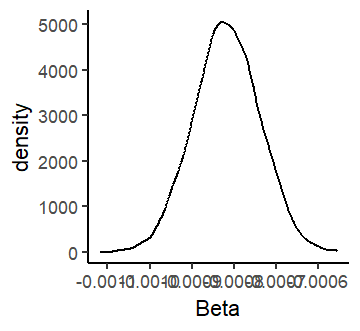
\includegraphics[width=\maxwidth]{figure/beta_dist-1} 

\end{knitrout}
\end{multicols}
\end{frame}

\begin{frame}
\frametitle{2. Regression as Conditional Expectation}
\begin{itemize}
\item How do we work out the conditional expectation? We estimate the $\beta$s
\item But we \textbf{NEVER} know the exact value of $\beta$
\item Regression \textbf{estimates a distribution} for each $\beta$
\begin{itemize}
\item That's why every $\beta$ comes with a standard error
\end{itemize}
\end{itemize}
\begin{multicols}{2}

% Table created by stargazer v.5.2.2 by Marek Hlavac, Harvard University. E-mail: hlavac at fas.harvard.edu
% Date and time: Thu, Mar 07, 2019 - 1:07:27 PM
\begin{table}[!htbp] \centering 
  \caption{} 
  \label{} 
\tiny 
\begin{tabular}{@{\extracolsep{1pt}}lc} 
\\[-1.8ex]\hline 
\hline \\[-1.8ex] 
 & \multicolumn{1}{c}{\textit{Dependent variable:}} \\ 
\cline{2-2} 
\\[-1.8ex] & redist \\ 
\hline \\[-1.8ex] 
 income & $-$0.000818$^{***}$ (0.000078) \\ 
  Constant & 2.234719$^{***}$ (0.361477) \\ 
 \hline \\[-1.8ex] 
Observations & 1,000 \\ 
\hline 
\hline \\[-1.8ex] 
\textit{Note:}  & \multicolumn{1}{r}{$^{*}$p$<$0.1; $^{**}$p$<$0.05; $^{***}$p$<$0.01} \\ 
\end{tabular} 
\end{table} 

\columnbreak
\begin{knitrout}
\definecolor{shadecolor}{rgb}{0.969, 0.969, 0.969}\color{fgcolor}
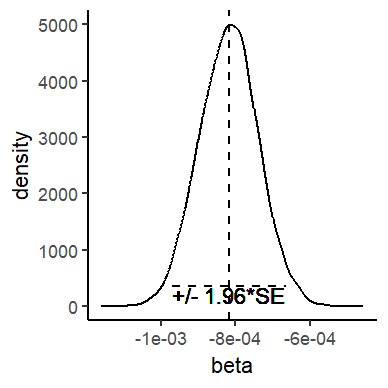
\includegraphics[width=\maxwidth]{figure/beta_dist_3-1} 

\end{knitrout}
\end{multicols}
\end{frame}

\begin{frame}
\frametitle{2. Regression as Conditional Expectation}
\begin{itemize}
\item How do we work out the conditional expectation? We estimate the $\beta$s
\item But we \textbf{NEVER} know the exact value of $\beta$
\item Regression \textbf{estimates a distribution} for each $\beta$
\begin{itemize}
\item That's why every $\beta$ comes with a standard error
\end{itemize}
\end{itemize}
\begin{multicols}{2}

% Table created by stargazer v.5.2.2 by Marek Hlavac, Harvard University. E-mail: hlavac at fas.harvard.edu
% Date and time: Thu, Mar 07, 2019 - 1:07:32 PM
\begin{table}[!htbp] \centering 
  \caption{} 
  \label{} 
\tiny 
\begin{tabular}{@{\extracolsep{1pt}}lc} 
\\[-1.8ex]\hline 
\hline \\[-1.8ex] 
 & \multicolumn{1}{c}{\textit{Dependent variable:}} \\ 
\cline{2-2} 
\\[-1.8ex] & redist \\ 
\hline \\[-1.8ex] 
 income & $-$0.000818$^{***}$ (0.000078) \\ 
  Constant & 2.234719$^{***}$ (0.361477) \\ 
 \hline \\[-1.8ex] 
Observations & 1,000 \\ 
\hline 
\hline \\[-1.8ex] 
\textit{Note:}  & \multicolumn{1}{r}{$^{*}$p$<$0.1; $^{**}$p$<$0.05; $^{***}$p$<$0.01} \\ 
\end{tabular} 
\end{table} 

\columnbreak
\begin{knitrout}
\definecolor{shadecolor}{rgb}{0.969, 0.969, 0.969}\color{fgcolor}
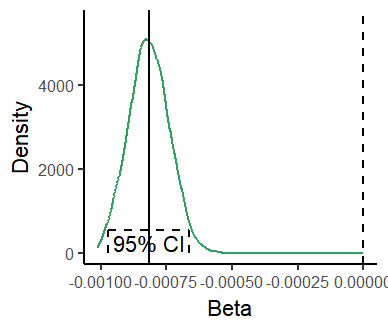
\includegraphics[width=\maxwidth]{figure/beta_dist_4-1} 

\end{knitrout}
\end{multicols}
\end{frame}

\begin{frame}
\frametitle{2. Regression as Conditional Expectation}
\begin{knitrout}
\definecolor{shadecolor}{rgb}{0.969, 0.969, 0.969}\color{fgcolor}
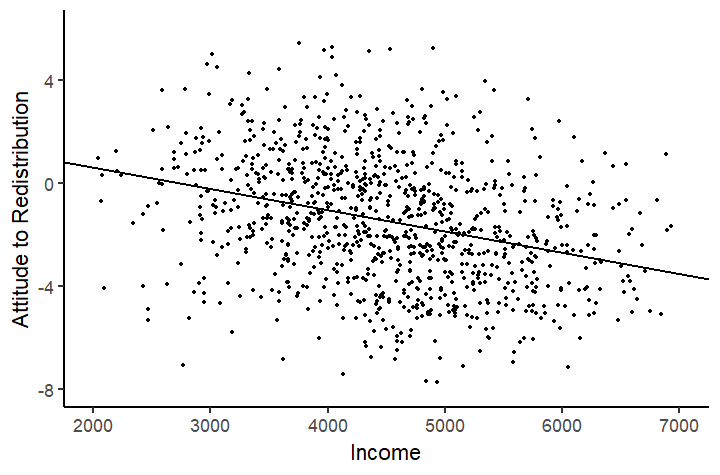
\includegraphics[width=\maxwidth]{figure/cond_exp1d-1} 

\end{knitrout}
\end{frame}

\begin{frame}
\frametitle{2. Regression as Conditional Expectation}
\begin{knitrout}
\definecolor{shadecolor}{rgb}{0.969, 0.969, 0.969}\color{fgcolor}
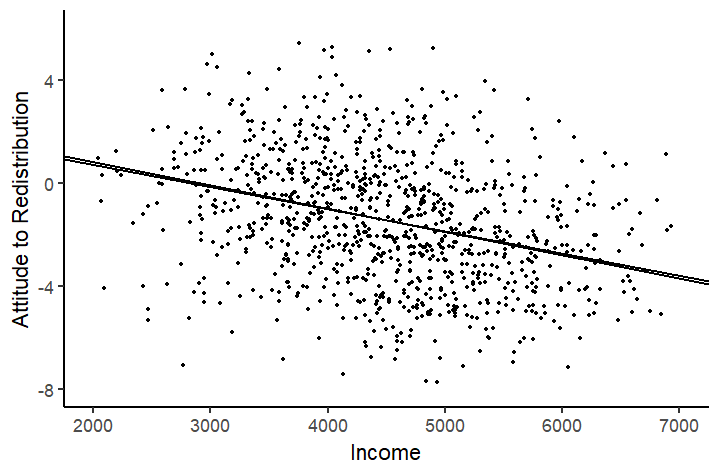
\includegraphics[width=\maxwidth]{figure/cond_exp1e-1} 

\end{knitrout}
\end{frame}

\begin{frame}
\frametitle{2. Regression as Conditional Expectation}
\begin{knitrout}
\definecolor{shadecolor}{rgb}{0.969, 0.969, 0.969}\color{fgcolor}
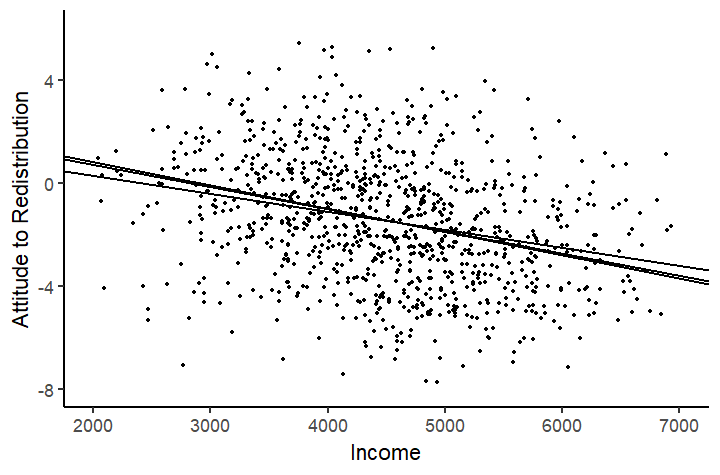
\includegraphics[width=\maxwidth]{figure/cond_exp1f-1} 

\end{knitrout}
\end{frame}

\begin{frame}
\frametitle{2. Regression as Conditional Expectation}
\begin{knitrout}
\definecolor{shadecolor}{rgb}{0.969, 0.969, 0.969}\color{fgcolor}
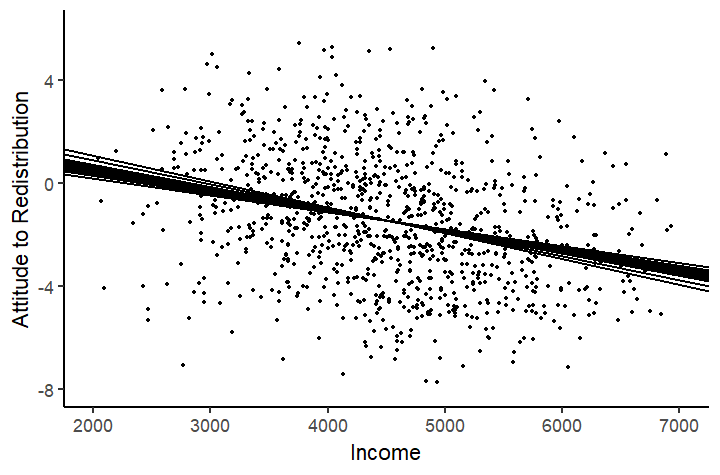
\includegraphics[width=\maxwidth]{figure/cond_exp1g-1} 

\end{knitrout}
\end{frame}

\begin{frame}
\frametitle{2. Regression as Conditional Expectation}
\begin{knitrout}
\definecolor{shadecolor}{rgb}{0.969, 0.969, 0.969}\color{fgcolor}
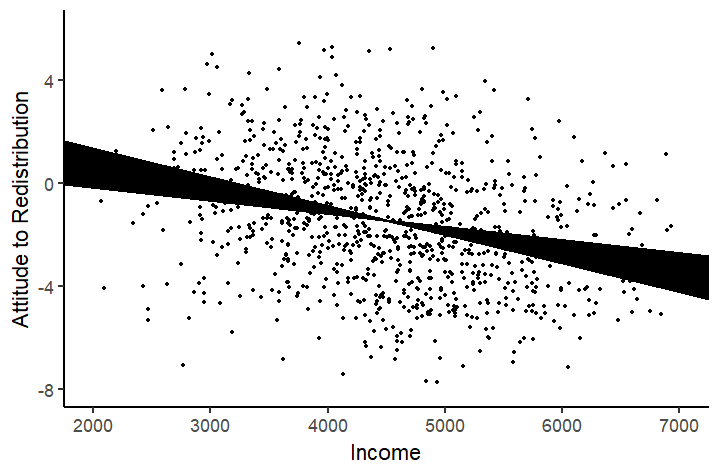
\includegraphics[width=\maxwidth]{figure/cond_exp1g2-1} 

\end{knitrout}
\end{frame}

\begin{frame}
\frametitle{2. Regression as Conditional Expectation}
\begin{knitrout}
\definecolor{shadecolor}{rgb}{0.969, 0.969, 0.969}\color{fgcolor}
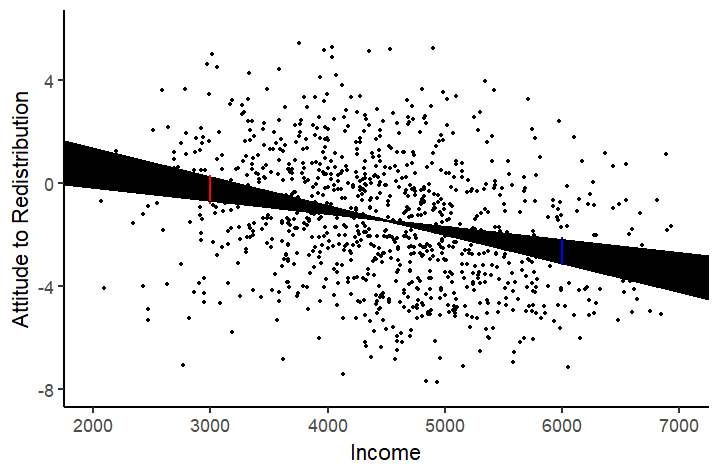
\includegraphics[width=\maxwidth]{figure/cond_exp1h-1} 

\end{knitrout}
\end{frame}

\begin{frame}
\frametitle{2. Regression as Conditional Expectation}
\begin{knitrout}
\definecolor{shadecolor}{rgb}{0.969, 0.969, 0.969}\color{fgcolor}
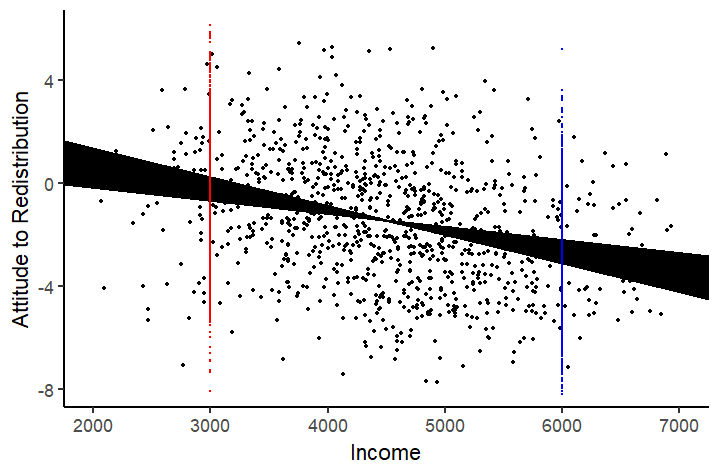
\includegraphics[width=\maxwidth]{figure/cond_exp1i-1} 

\end{knitrout}
\end{frame}




\begin{frame}
\frametitle{3. Regression as (Partial) Correlation}
\begin{itemize}
\item Regression with two variables is very similar to calculating correlation:
\pause
\item $\hat{\beta}=cor(x,y) * \frac{\sigma_Y}{\sigma_X}$
\pause
\end{itemize}
\begin{multicols}{2}
\begin{knitrout}
\definecolor{shadecolor}{rgb}{0.969, 0.969, 0.969}\color{fgcolor}
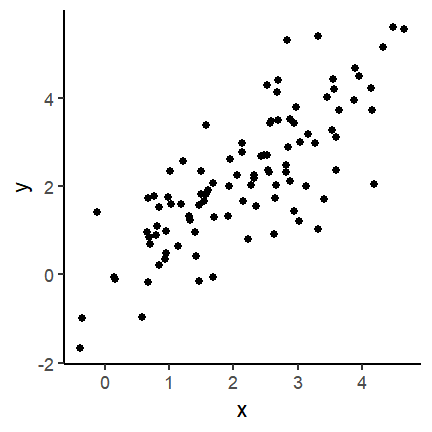
\includegraphics[width=\maxwidth]{figure/corr_regn_fig1-1} 

\end{knitrout}
\columnbreak
\end{multicols}
\end{frame}

\begin{frame}
\frametitle{3. Regression as (Partial) Correlation}
\begin{itemize}
\item Regression with two variables is very similar to calculating correlation:
\item $\hat{\beta}=cor(x,y) * \frac{\sigma_Y}{\sigma_X}$
\end{itemize}
\begin{multicols}{2}
\begin{knitrout}
\definecolor{shadecolor}{rgb}{0.969, 0.969, 0.969}\color{fgcolor}
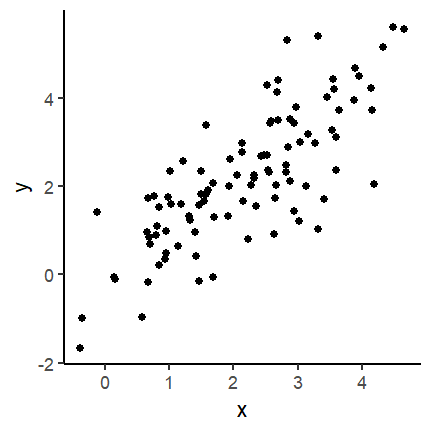
\includegraphics[width=\maxwidth]{figure/corr_regn_fig2-1} 

\end{knitrout}
\columnbreak
\begin{itemize}
\item Correlation is 0.781
\pause
\item Regression Results:
\end{itemize}
% latex table generated in R 3.5.2 by xtable 1.8-3 package
% Sat Mar 02 10:51:08 2019
\begin{table}[ht]
\centering
\begin{tabular}{rlr}
  \hline
 & term & estimate \\ 
  \hline
1 & (Intercept) & 0.006 \\ 
  2 & x & 1.008 \\ 
   \hline
\end{tabular}
\end{table}

\end{multicols}
\end{frame}

\begin{frame}
\frametitle{3. Regression as (Partial) Correlation}
\begin{itemize}
\item Regression with two variables is very similar to calculating correlation:
\item $\hat{\beta}=cor(x,y) * \frac{\sigma_Y}{\sigma_X}$
\end{itemize}
\begin{multicols}{2}
\begin{knitrout}
\definecolor{shadecolor}{rgb}{0.969, 0.969, 0.969}\color{fgcolor}
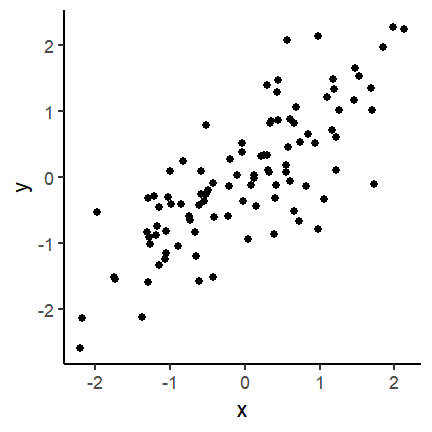
\includegraphics[width=\maxwidth]{figure/corr_regn_fig3-1} 

\end{knitrout}
\columnbreak
\begin{itemize}
\item Correlation is 0.781
\item It's \textbf{identical} if we standardize both variables first ($\frac{(x_i-\bar{x})}{\sigma_x}$)
\item Standardized Regression Results:
\end{itemize}
% latex table generated in R 3.5.2 by xtable 1.8-3 package
% Sat Mar 02 10:51:11 2019
\begin{table}[ht]
\centering
\begin{tabular}{rlr}
  \hline
 & term & estimate \\ 
  \hline
1 & (Intercept) & 0.000 \\ 
  2 & x & 0.781 \\ 
   \hline
\end{tabular}
\end{table}

\end{multicols}
\end{frame}

\begin{frame}
\frametitle{3. Regression as (Partial) Correlation}
\begin{itemize}
\item Regression with \textbf{multiple} variables is very similar to calculating \textbf{partial} correlation
\pause
\item $y_i = \alpha + \beta_1 x_1 + \beta_2 x_2 +\epsilon_i$
\pause
\item Just a small difference in the denominator (how we standardize the measure)
\pause
\end{itemize}
$$\beta_{x_1} = \frac{r_{yx_1} - r_{yx_2}r_{x_1x_2}}{1-r^2_{x_1x_2}}$$
$$r_{yx_1|x_2} = \frac{r_{yx_1} - r_{yx_2}r_{x_1x_2}}{\sqrt{(1-r^2_{yx_2})(1-r^2_{x_1x_2})}}$$
\begin{itemize}
\item \textbf{There is no magic in regression, it's just 'extra' correlation}
\end{itemize}
\end{frame}



\section{Guide to 'Smart' Regression}

\begin{frame}
\frametitle{Regression Guide}
\begin{enumerate}
\item We will use regression throughout this course
\pause
\item But in a very \textbf{precise} way for each methodology
\pause
\item There are fundamental best practices that apply to all the methodologies
\end{enumerate}
\end{frame}

\begin{frame}
\frametitle{Regression Guide}
\begin{enumerate}
\item \textbf{Choose Variables and Measures:} To test a specific hypothesis
\pause
\item \textbf{Choose the Data:} Throw out data we cannot learn from!
\pause
\item \textbf{Choose a Model/Link Function:} To match the data type of your outcome variable
\pause
\item \textbf{Choose Covariates:} To make specific comparisons
\pause
\item \textbf{Choose Fixed Effects:} To focus on comparisons at a specific level
\pause
\item \textbf{Choose Error Structure:} To match known dependencies/clustering in the data or sampling
\pause
\item \textbf{Interpret the Coefficients:} To match the type/scale of the explanatory variable, outcome variable and model
\pause
\item \textbf{Predict Meaningful Comparisons:} To communicate your findings
\end{enumerate}
\end{frame}

\begin{frame}
\frametitle{1. Variables and Measures}
\begin{itemize}
\item For the research question ``Does income affect attitudes to redistribution?''
\pause
\item What measure of income should we use?
\pause
\begin{itemize}
\item Pre-tax, post-tax, after government benefits?
\end{itemize}
\item It depends on the theory we are testing
\end{itemize}
\end{frame}

\begin{frame}
\frametitle{2. Data Sample}
\begin{itemize}
\item For the research question ``Does income affect attitudes to redistribution?''
\pause
\item We are conducting a within-country analysis
\pause
\item But everyone in our data from Qatar earns exactly \$1m - no variation in income!
\pause
\item We may as well throw the Qatar data away
\end{itemize}
\end{frame}

\begin{frame}
\frametitle{3. Regression Models}
The Regression Model reflects the data type of the outcome variable:
\begin{itemize}
\item Continuous -> Ordinary Least Squares  
\begin{itemize}
\item ``Pick a precise number that reflects your attitude to redistribution''
\end{itemize}
\pause
\item Binary -> Logit  
\begin{itemize}
\item ``Do you support redistribution, yes or no?''
\end{itemize}
\pause
\item Unordered categories -> Multinomial logit  
\begin{itemize}
\item ``Do you think redistribution is a western, oriental or african concept?''
\end{itemize}
\pause
\item Ordered categories -> Ordered logit  
\begin{itemize}
\item ``Do you want a lot more, more, the same, less, or a lot less redistribution?''
\end{itemize}
\pause
\item Count -> Poisson  
\begin{itemize}
\item ``In the past year, how many times have you complained about redistribution?''
\end{itemize}
\end{itemize}
\end{frame}

\begin{frame}
\frametitle{4. Covariates}
\begin{itemize}
\item Which covariates should we include?
\pause
\item Which comparisons do we want to make?
\pause
\item Control for gender if we want to compare men with men, women with women
\pause
\item Only include controls where there is theory or evidence that this variable could be an \textbf{omitted variable}
\pause
\item Controlling for post-treatment variables can make your estimate \textit{worse}
\end{itemize}
\end{frame}

\begin{frame}
\frametitle{5. Fixed Effects}
\begin{itemize}
\item Data are usually hierarchical: countries, states, municipalities, neighbourhoods, families, individuals
\pause
\item A fixed effect for countries means we only compare people within the same country
\pause
\item Removing \textit{ALL} the variation between countries
\begin{itemize}
\item If rich \textit{countries} have stronger attitudes to redistribution, we control for this
\item So we can ask whether richer \textit{people} have stronger attitudes
\end{itemize}
\pause
\item Our question becomes: How do variations within income in the same country affect attitudes to redistribution?
\end{itemize}
\end{frame}

\begin{frame}
\frametitle{6. Errors Structure}
\begin{itemize}
\item An assumption of regression analysis is that the errors are independent
\pause
\begin{itemize}
\item Knowing the value of one error tells you \textit{nothing} about the value of the next error
\end{itemize}
\pause
\item But attitudes to redistribution are probably very similar to everyone you live with, even after controlling for income etc. 
\pause
\item Due to 'unobservable' variables (conversations over dinner...)
\pause
\item So we don't really have 2 observations, we have closer to 1 'independent' observation
\pause
\item So the standard errors for our $\beta$'s are \textit{over-confident} (too small)
\pause
\item We need to adjust for these dependencies with clustered standard errors
\begin{itemize}
\item Created by the underlying structure of the data
\item Or by our data sampling process
\end{itemize}
\end{itemize}
\end{frame}

\begin{frame}
\frametitle{6. Errors Structure}
\begin{multicols}{2}
\begin{knitrout}
\definecolor{shadecolor}{rgb}{0.969, 0.969, 0.969}\color{fgcolor}
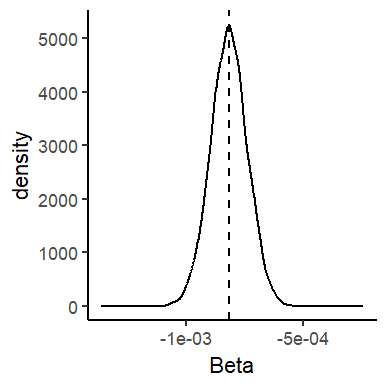
\includegraphics[width=\maxwidth]{figure/beta_dist_errors_4-1} 

\end{knitrout}
\columnbreak
\begin{itemize}
\item The distribution of our estimated betas suggests we're pretty confident $\beta$ is close to $-0.0008175$
\end{itemize}
\end{multicols}
\end{frame}

\begin{frame}
\frametitle{6. Errors Structure}
\begin{multicols}{2}
\begin{knitrout}
\definecolor{shadecolor}{rgb}{0.969, 0.969, 0.969}\color{fgcolor}
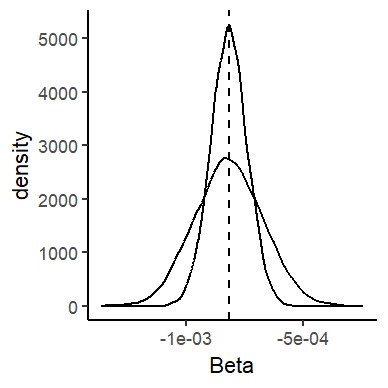
\includegraphics[width=\maxwidth]{figure/beta_dist_errors_5-1} 

\end{knitrout}
\columnbreak
\begin{itemize}
\item With clustered SEs, the wider distribution of our betas suggests we're \textit{less} confident $\beta$ is close to $-0.0008175$
\end{itemize}
\end{multicols}
\end{frame}

\begin{frame}
\frametitle{7. Interpreting Regression Results}
\begin{itemize}
\item Difficult! It depends on:
\begin{enumerate}
\item The scale of the explanatory variable
\pause
\item The scale of the outcome
\pause
\item The regression model we used
\pause
\item The presence of any interaction
\pause
\end{enumerate}
\item Basic OLS: $y_i = \alpha + \beta D_i + \epsilon$
\pause
\begin{itemize}
\item A \textcolor{blue}{1 [unit of $D$]} change in the explanatory variable is associated with a \textcolor{blue}{$\beta$ [unit of $y$]} change in the outcome, holding other variables constant
\end{itemize}
\end{itemize}
\end{frame}

\begin{frame}
\frametitle{7. Interpreting Regression Results}
\begin{itemize}
\item Difficult! It depends on:
\begin{enumerate}
\item The scale of the explanatory variable
\item The scale of the outcome
\item The regression model we used
\item The presence of any interaction
\end{enumerate}
\item Basic OLS \textbf{with log outcome}: $log(y_i) = \alpha + \beta D_i + \epsilon$
\begin{itemize}
\item A \textcolor{blue}{1 [unit of $D$]} change in the explanatory variable is associated with a  \textcolor{blue}{$100*(e^{\beta}-1)\%$} change in the outcome, holding other variables constant
\end{itemize}
\end{itemize}
\end{frame}

\begin{frame}
\frametitle{7. Interpreting Regression Results}
\begin{itemize}
\item Difficult! It depends on:
\begin{enumerate}
\item The scale of the explanatory variable
\item The scale of the outcome
\item The regression model we used
\item The presence of any interaction
\end{enumerate}
\item Basic OLS \textbf{with log treatment}: $y_i = \alpha + \beta log(D_i) + \epsilon$
\begin{itemize}
\item A \textcolor{blue}{1\%} change in the explanatory variable is associated with a  \textcolor{blue}{$\beta*log(\frac{101}{100})$} change in the outcome, holding other variables constant
\end{itemize}
\end{itemize}
\end{frame}

\begin{frame}
\frametitle{7. Interpreting Regression Results}
\begin{itemize}
\item Difficult! It depends on:
\begin{enumerate}
\item The scale of the explanatory variable
\item The scale of the outcome
\item The regression model we used
\item The presence of any interaction
\end{enumerate}
\item \textbf{Logit:} $log(\frac{Pr(y_i=1)}{Pr(y_i=0)}) = \alpha + \beta D_i + \epsilon$
\begin{itemize}
\item A \textcolor{blue}{1 [unit of $D$]} change in the explanatory variable is associated with a \textcolor{blue}{$\beta$ change in the log-odds} of $y_i=1$, holding other variables constant
\end{itemize}
\end{itemize}
\end{frame}

\begin{frame}
\frametitle{7. Interpreting Regression Results}
\begin{itemize}
\item Difficult! It depends on:
\begin{enumerate}
\item The scale of the explanatory variable
\item The scale of the outcome
\item The regression model we used
\item The presence of any interaction
\end{enumerate}
\item \textbf{Logit:} $log(\frac{Pr(y_i=1)}{Pr(y_i=0)}) = \alpha + \beta D_i + \epsilon$
\begin{itemize}
\item A \textcolor{blue}{1 [unit of $D$]} change in the explanatory variable is associated with a \textcolor{blue}{$100*(e^{\beta}-1)\%$ change in the odds (relative probability, $\frac{p}{1-p}$)} of $y_i=1$, holding other variables constant
\end{itemize}
\end{itemize}
\end{frame}

\begin{frame}
\frametitle{7. Interpreting Regression Results}
\begin{itemize}
\item Difficult! It depends on:
\begin{enumerate}
\item The scale of the explanatory variable
\item The scale of the outcome
\item The regression model we used
\item The presence of any interaction
\end{enumerate}
\item \textbf{Multinomial:} $log(\frac{Pr(y_i=C)}{Pr(y_i=B)}) = \alpha + \beta D_i + \epsilon$
\begin{itemize}
\item A \textcolor{blue}{1 [unit of $D$]} change in the explanatory variable is associated with a \textcolor{blue}{$100*(e^{\beta_C}-1)\%$ change in the odds (relative probability, $\frac{p}{1-p}$)} of moving from the baseline category $B$ to the outcome category $C$, holding other variables constant
\end{itemize}
\end{itemize}
\end{frame}

\begin{frame}
\frametitle{7. Interpreting Regression Results}
\begin{itemize}
\item Difficult! It depends on:
\begin{enumerate}
\item The scale of the explanatory variable
\item The scale of the outcome
\item The regression model we used
\item The presence of any interaction
\end{enumerate}
\item \textbf{Ordered Multinomial:} $log(\frac{Pr(y_i=C)}{Pr(y_i=C-1)}) = \alpha + \beta D_i + \epsilon$
\begin{itemize}
\item A \textcolor{blue}{1 [unit of $D$]} change in the explanatory variable is associated with a \textcolor{blue}{$100*(e^{\beta}-1)\%$ change in the odds (relative probability, $\frac{p}{1-p}$)} of moving up one unit on the outcome scale, holding other variables constant
\end{itemize}
\end{itemize}
\end{frame}

\begin{frame}
\frametitle{7. Interpreting Regression Results}
\begin{itemize}
\item Difficult! It depends on:
\begin{enumerate}
\item The scale of the explanatory variable
\item The scale of the outcome
\item The regression model we used
\item The presence of any interaction
\end{enumerate}
\item \textbf{OLS with Interaction:} $y_i = \alpha + \beta_1 D_i + \beta_2 X_i + \beta_3 D_i * X_i + \epsilon$
\begin{itemize}
\item $ \frac{\partial y}{\partial D} = \beta_1 + \beta_3 X$
\item \textcolor{blue}{$\beta_1$ is the effect of $D$ when $X=0$} : \textit{May not make sense!}
\item Insert values for $X$ and see how the marginal effect changes
\end{itemize}
\end{itemize}
\end{frame}

\begin{frame}
\frametitle{7. Interpreting Regression Results}
\begin{multicols}{2}
\footnotesize
\textbf{OLS with Interaction:} \\
$$Redist_i = \alpha + \beta_1 Gender_i + \beta_2 Income_i \\+ \beta_3 Gender_i * Income_i + \epsilon_i$$ \\
\pause
$$\frac{\partial Redist}{\partial Gender} = \beta_1 + \beta_3*Income$$ \\
\pause
$$\frac{\partial Redist}{\partial Income} = \beta_2 + \beta_3*Gender$$
\normalsize
\pause

% Table created by stargazer v.5.2.2 by Marek Hlavac, Harvard University. E-mail: hlavac at fas.harvard.edu
% Date and time: Thu, Mar 21, 2019 - 10:56:54 AM
\begin{table}[!htbp] \centering 
  \caption{} 
  \label{} 
\tiny 
\begin{tabular}{@{\extracolsep{1pt}}lc} 
\\[-1.8ex]\hline 
\hline \\[-1.8ex] 
 & \multicolumn{1}{c}{\textit{Dependent variable:}} \\ 
\cline{2-2} 
\\[-1.8ex] & redist \\ 
\hline \\[-1.8ex] 
 gender1 & $-$2.942614$^{***}$ (0.700510) \\ 
  income & 0.079980$^{***}$ (0.000110) \\ 
  gender1:income & 0.000986$^{***}$ (0.000152) \\ 
  Constant & 0.112903 (0.454926) \\ 
 \hline \\[-1.8ex] 
Observations & 1,000 \\ 
\hline 
\hline \\[-1.8ex] 
\textit{Note:}  & \multicolumn{1}{r}{$^{*}$p$<$0.1; $^{**}$p$<$0.05; $^{***}$p$<$0.01} \\ 
\end{tabular} 
\end{table} 

\columnbreak
\pause
\begin{knitrout}
\definecolor{shadecolor}{rgb}{0.969, 0.969, 0.969}\color{fgcolor}
\includegraphics[width=\maxwidth]{figure/interaction_plot_2-1} 

\end{knitrout}
\pause
\begin{knitrout}
\definecolor{shadecolor}{rgb}{0.969, 0.969, 0.969}\color{fgcolor}
\includegraphics[width=\maxwidth]{figure/interaction_plot_3-1} 

\end{knitrout}
\end{multicols}
\end{frame}

\begin{frame}
\frametitle{8. Predictions from Regressions}
\begin{itemize}
\item The coefficient on the regression of income on attitude to redistribution is -0.000818
\begin{itemize}
\pause
\item So??? What do we learn from this?
\pause
\item Coefficients are hard to interpret, and depend on how we measure each variable
\item And p-values are arbitrary (0.049 vs. 0.051)
\end{itemize}  
\pause
\item Better to make specific \textit{predictions} of how changes in $D$ produce changes in $Y$
\end{itemize}
\end{frame}

\begin{frame}
\frametitle{8. Predictions from Regressions}
$$Attitude_i = \alpha + \beta_1 \text{ Income}_i + \epsilon_i$$ \\
\pause
$$Attitude_i = 2.235 - 0.000818 \text{ Income}_i + N(0,2.378)$$ \\
\pause
\textbf{If Income is 3000:}  \\
$$Attitude_i = 2.235-0.000818*3000 + N(0,2.378)$$ \\
$$Attitude_i = -0.219 + N(0,2.378)$$
\end{frame}

\begin{frame}
\frametitle{8. Predictions from Regressions}
$$Attitude_i = \alpha + \beta_1 \text{ Income}_i + \epsilon_i$$ \\
$$Attitude_i = 2.235 - 0.000818 \text{ Income}_i + N(0,2.378)$$ \\
\textbf{If Income is 6000:}  \\
$$Attitude_i = 2.235-0.000818*6000 + N(0,2.378)$$ \\
$$Attitude_i = -2.673 + N(0,2.378)$$
\end{frame}

\begin{frame}
\frametitle{8. Predictions from Regressions}
$$Attitude_i = \alpha + \beta_1 \text{ Income}_i + \epsilon_i$$
$$Attitude_i = 2.235 - 0.000818 \text{ Income}_i + N(0,2.378)$$
\textbf{Increasing Income from 3000 to 6000:} \\
$$\Delta Attitude_i = (2.235-0.000818*6000) - (2.235-0.000818*3000)$$
$$\Delta Attitude_i = -2.673 - (-0.219)$$
$$\Delta Attitude_i = -2.454$$
\end{frame}

\begin{frame}
\frametitle{8. Predictions from Regressions}
\begin{knitrout}
\definecolor{shadecolor}{rgb}{0.969, 0.969, 0.969}\color{fgcolor}
\includegraphics[width=\maxwidth]{figure/predictions1-1} 

\end{knitrout}
\end{frame}

\begin{frame}
\frametitle{8. Predictions from Regressions}
\begin{multicols}{2}
Predicted Values:
\begin{knitrout}
\definecolor{shadecolor}{rgb}{0.969, 0.969, 0.969}\color{fgcolor}
\includegraphics[width=\maxwidth]{figure/predictions2-1} 

\end{knitrout}
\columnbreak
\pause
First Differences:
\begin{knitrout}
\definecolor{shadecolor}{rgb}{0.969, 0.969, 0.969}\color{fgcolor}
\includegraphics[width=\maxwidth]{figure/predictions3-1} 

\end{knitrout}
\end{multicols}
\end{frame}

\begin{frame}
\frametitle{8. Predictions from Regressions}
\begin{itemize}
\item The regression model matters because the wrong model makes non-sensical predictions
\pause
\item Consider a binary outcome: $Gender_i = \alpha + \beta Income_i + \epsilon_i$
\pause
\item Compare the OLS and Logit regression tables:
\pause
\end{itemize}
\begin{multicols}{2}

% Table created by stargazer v.5.2.2 by Marek Hlavac, Harvard University. E-mail: hlavac at fas.harvard.edu
% Date and time: Thu, Mar 21, 2019 - 11:12:10 AM
\begin{table}[!htbp] \centering 
  \caption{} 
  \label{} 
\tiny 
\begin{tabular}{@{\extracolsep{1pt}}lc} 
\\[-1.8ex]\hline 
\hline \\[-1.8ex] 
 & \multicolumn{1}{c}{\textit{Dependent variable:}} \\ 
\cline{2-2} 
\\[-1.8ex] & gender \\ 
\hline \\[-1.8ex] 
 income & 0.0003$^{***}$ (0.00001) \\ 
  Constant & $-$0.696$^{***}$ (0.066) \\ 
 \hline \\[-1.8ex] 
Observations & 1,000 \\ 
\hline 
\hline \\[-1.8ex] 
\textit{Note:}  & \multicolumn{1}{r}{$^{*}$p$<$0.1; $^{**}$p$<$0.05; $^{***}$p$<$0.01} \\ 
\end{tabular} 
\end{table} 

\columnbreak

% Table created by stargazer v.5.2.2 by Marek Hlavac, Harvard University. E-mail: hlavac at fas.harvard.edu
% Date and time: Thu, Mar 21, 2019 - 11:12:11 AM
\begin{table}[!htbp] \centering 
  \caption{} 
  \label{} 
\tiny 
\begin{tabular}{@{\extracolsep{1pt}}lc} 
\\[-1.8ex]\hline 
\hline \\[-1.8ex] 
 & \multicolumn{1}{c}{\textit{Dependent variable:}} \\ 
\cline{2-2} 
\\[-1.8ex] & gender \\ 
\hline \\[-1.8ex] 
 income & 0.001$^{***}$ (0.0001) \\ 
  Constant & $-$6.360$^{***}$ (0.457) \\ 
 \hline \\[-1.8ex] 
Observations & 1,000 \\ 
\hline 
\hline \\[-1.8ex] 
\textit{Note:}  & \multicolumn{1}{r}{$^{*}$p$<$0.1; $^{**}$p$<$0.05; $^{***}$p$<$0.01} \\ 
\end{tabular} 
\end{table} 

\end{multicols}
\end{frame}

\begin{frame}
\frametitle{8. Predictions from Regressions}
\begin{itemize}
\item The regression model matters because the wrong model makes non-sensical predictions
\item Consider a binary outcome: $Gender_i = \alpha + \beta Income_i + \epsilon_i$
\item Compare the OLS and Logit \textbf{predictions} of gender for an income of R\$3000:
\end{itemize}
\begin{multicols}{2}
\begin{knitrout}
\definecolor{shadecolor}{rgb}{0.969, 0.969, 0.969}\color{fgcolor}
\includegraphics[width=\maxwidth]{figure/preds_1_ols_chart-1} 

\end{knitrout}
\columnbreak
\begin{knitrout}
\definecolor{shadecolor}{rgb}{0.969, 0.969, 0.969}\color{fgcolor}
\includegraphics[width=\maxwidth]{figure/preds_1_logit_chart-1} 

\end{knitrout}
\end{multicols}
\end{frame}

\section{What Does Regression NOT Do?}

\begin{frame}
\frametitle{What Does Regression NOT Do?}
\begin{itemize}
\item Remember, regression is just fancy correlation
\pause
\item Even after following all this guidance, Regression does NOT:
\begin{enumerate}
\item \textit{Explain} anything
\item Make bad data better
\item Tell you which theory is 'correct'
\item Make it clear what comparisons you are making
\end{enumerate}
\pause
\item These all require \textbf{research design}, \textbf{theory} and \textbf{assumptions}
\end{itemize}
\end{frame}

\begin{frame}
\frametitle{What Does Regression NOT Do?}
\begin{itemize}
\item \textbf{Correlation is not causation}
\pause
\begin{itemize}
\item If we look hard enough we can always find correlations
\pause
\item By chance...
\pause
\item Due to complex social and historical patterns...
\pause
\item But we cannot conclude that $D$ causes or explains $Y$
\pause
\end{itemize}
\item \textit{More} data will not help
\pause
\item The problem is the \textit{content} of data; it does not allow us to answer the causal question 
\end{itemize}
\end{frame}

\setbeamercolor{background canvas}{bg=}
\includegraphics[width=0.85\textwidth]{Chocolate_Nobel.jpg}

\setbeamercolor{background canvas}{bg=}
\includepdf[pages={1}]{chart_1.pdf}

\setbeamercolor{background canvas}{bg=}
\includepdf[pages={1}]{chart_2.pdf}

\setbeamercolor{background canvas}{bg=}
\includepdf[pages={1}]{chart_3.pdf}

\setbeamercolor{background canvas}{bg=}
\includepdf[pages={1}]{chart_4.pdf}

\begin{frame}
\frametitle{What Does Regression NOT Do?}
\begin{itemize}
\item Why is correlation (regression) not causation?
\pause
\begin{enumerate}
\item Omitted Variable Bias
\pause
\item Reverse Causation
\pause
\item Selection Bias
\pause
\item Measurement Bias
\pause
\item Lack of Overlap, Model Dependence
\end{enumerate}
\end{itemize}
\end{frame}

\begin{frame}
\frametitle{1. Omitted Variable Bias}
\begin{knitrout}
\definecolor{shadecolor}{rgb}{0.969, 0.969, 0.969}\color{fgcolor}
\includegraphics[width=\maxwidth]{figure/confound3b-1} 

\end{knitrout}
\end{frame}

\begin{frame}
\frametitle{1. Omitted Variable Bias}
\begin{knitrout}
\definecolor{shadecolor}{rgb}{0.969, 0.969, 0.969}\color{fgcolor}
\includegraphics[width=\maxwidth]{figure/confound3c-1} 

\end{knitrout}
\end{frame}

\begin{frame}
\frametitle{1. Omitted Variable Bias}
\begin{knitrout}
\definecolor{shadecolor}{rgb}{0.969, 0.969, 0.969}\color{fgcolor}
\includegraphics[width=\maxwidth]{figure/confound2-1} 

\end{knitrout}
\end{frame}


\begin{frame}
\frametitle{1. Omitted Variable Bias}
\begin{knitrout}
\definecolor{shadecolor}{rgb}{0.969, 0.969, 0.969}\color{fgcolor}
\includegraphics[width=\maxwidth]{figure/confound3-1} 

\end{knitrout}
\end{frame}

\begin{frame}
\frametitle{2. Reverse Causation}
\begin{itemize}
\item Significant regression coefficients just reflect the values in our dataset moving together
\pause
\item Does the 'direction' of regression  matter? I.e. Does regression treat $D$ and $Y$ differently? \pause Yes! 
\end{itemize}
\begin{multicols}{2}

% Table created by stargazer v.5.2.2 by Marek Hlavac, Harvard University. E-mail: hlavac at fas.harvard.edu
% Date and time: Wed, Mar 06, 2019 - 12:10:54 PM
\begin{table}[!htbp] \centering 
  \caption{} 
  \label{} 
\tiny 
\begin{tabular}{@{\extracolsep{1pt}}lc} 
\\[-1.8ex]\hline 
\hline \\[-1.8ex] 
 & \multicolumn{1}{c}{\textit{Dependent variable:}} \\ 
\cline{2-2} 
\\[-1.8ex] & redist \\ 
\hline \\[-1.8ex] 
 income & $-$0.011 (0.029) \\ 
  gender1 & $-$1.201$^{***}$ (0.058) \\ 
  Constant & 0.589$^{***}$ (0.038) \\ 
 \hline \\[-1.8ex] 
Observations & 1,000 \\ 
\hline 
\hline \\[-1.8ex] 
\textit{Note:}  & \multicolumn{1}{r}{$^{*}$p$<$0.1; $^{**}$p$<$0.05; $^{***}$p$<$0.01} \\ 
\end{tabular} 
\end{table} 

\columnbreak

% Table created by stargazer v.5.2.2 by Marek Hlavac, Harvard University. E-mail: hlavac at fas.harvard.edu
% Date and time: Wed, Mar 06, 2019 - 12:10:55 PM
\begin{table}[!htbp] \centering 
  \caption{} 
  \label{} 
\tiny 
\begin{tabular}{@{\extracolsep{1pt}}lc} 
\\[-1.8ex]\hline 
\hline \\[-1.8ex] 
 & \multicolumn{1}{c}{\textit{Dependent variable:}} \\ 
\cline{2-2} 
\\[-1.8ex] & income \\ 
\hline \\[-1.8ex] 
 redist & $-$0.013 (0.034) \\ 
  gender1 & 0.993$^{***}$ (0.069) \\ 
  Constant & $-$0.487$^{***}$ (0.043) \\ 
 \hline \\[-1.8ex] 
Observations & 1,000 \\ 
\hline 
\hline \\[-1.8ex] 
\textit{Note:}  & \multicolumn{1}{r}{$^{*}$p$<$0.1; $^{**}$p$<$0.05; $^{***}$p$<$0.01} \\ 
\end{tabular} 
\end{table} 

\end{multicols}
\pause
\begin{itemize}
\item Remember, regression measures the \textit{vertical} (not diagonal) distances to the regression line
\begin{itemize}
\item It minimizes the \textit{prediction errors} for $Y$
\end{itemize}
\pause
\item But that doesn't mean it identifies the direction of causation!
\end{itemize}
\end{frame}

\begin{frame}
\frametitle{2. Reverse Causation}
\begin{itemize}
\item Higher income may lead to higher tax payments and therefore cause more negative attitudes to redistribution
\pause
\item But negative attitudes to redistribution might also make you more likely to work in the private sector and cause you to receive a higher salary
\pause
\item Both would look the same in a regression
\pause
\item We cannot \textit{explain} the relationship with a regression
\end{itemize}
\end{frame}

\begin{frame}
\frametitle{3. Selection Bias}
\begin{itemize}
\item Imagine we do not see 'rich' units with high income (above R\$4000)
\end{itemize}
\begin{knitrout}
\definecolor{shadecolor}{rgb}{0.969, 0.969, 0.969}\color{fgcolor}
\includegraphics[width=\maxwidth]{figure/selection1-1} 

\end{knitrout}
\end{frame}

\begin{frame}
\frametitle{3. Selection Bias}
\begin{itemize}
\item Imagine we do not see 'rich' units with high income (above R\$4000)
\end{itemize}
\begin{knitrout}
\definecolor{shadecolor}{rgb}{0.969, 0.969, 0.969}\color{fgcolor}
\includegraphics[width=\maxwidth]{figure/selection2-1} 

\end{knitrout}
\end{frame}

\begin{frame}
\frametitle{3. Selection Bias}
\begin{itemize}
\item There are four selection risks:
\begin{enumerate}
\item \textbf{Selection into existence}
\item \textbf{Selection into survival}
\item \textbf{Selection into the dataset}
\item \textbf{Selection into treatment}
\end{enumerate}
\pause
\item In each case, we don't see the \textit{full} relationship between $D$ and $Y$
\pause
\item So our regression estimates are biased
\end{itemize}
\end{frame}

\begin{frame}
\frametitle{3. Selection Bias}
\begin{itemize}
\item There are four selection risks:
\begin{itemize}
\item \textbf{1. Selection into existence:}
\pause
\begin{itemize}
\item Where do units (eg. political parties) come from?
\pause
\item Probably only parties that have a chance of success are formed
\pause
\item Does forming a party cause electoral success? Not for most people!
\end{itemize}
\end{itemize}
\end{itemize}
\end{frame}

\begin{frame}
\frametitle{3. Selection Bias}
\begin{itemize}
\item There are four selection risks:
\begin{itemize}
\item \textbf{2. Selection into survival:}
\pause
\begin{itemize}
\item Certain types of units disappear, so the units we see don't tell the full story
\end{itemize}
\pause
\end{itemize}
\end{itemize}
\begin{multicols}{2}
\includegraphics[scale=0.25]{Bombers.pdf}
\columnbreak
\begin{itemize}
\item Where would additional armour protect bombers?
\pause
\item Returned bombers got hit
\pause
\item But we do not know where \textit{bombers that did not return} got hit
\end{itemize}
\end{multicols}
\end{frame}

\begin{frame}
\begin{itemize}
\item test
\begin{itemize}
\item test
\begin{enumerate}
\item test
\item test2
\begin{itemize}
\item shuold be in item
\end{itemize}
\item test3 enum
\end{itemize}
\end{enumerate}
\end{itemize}
\end{frame}

\begin{frame}
\frametitle{Summary}
\begin{enumerate}
\item Regression is just fancy correlation
\begin{itemize}
\item A \textbf{conditional expectation function}
\pause
\end{itemize}
\item 'Smart' regression pays more attention to what \textbf{comparisons} you want to make than to statistical tests
\begin{itemize}
\item And to \textbf{interpretation/prediction} rather than p-values
\end{itemize}
\pause
\item Regression \textbf{cannot explain} relationships
\begin{itemize}
\item \textbf{Correlation is not causation}
\pause
\item We need to understand better \textbf{how the data were produced}
\pause
\item \textbf{Explanation} depends on research design, data selection, assumptions and qualitative evidence
\end{itemize}
\end{enumerate}
\end{frame}

\end{document}


%setwd('C:\\Users\\Jonny\\Google Drive\\Academic\\USP\\Class\\Week 1 - Intro\\Lecture Slides')
%knitr::knit("Slides_Wk1_intro_5.Rnw")
